%!TEX root = ../thesis.tex
\chapter{盾构隧道服役性能评估方法}

在道路工程领域,同样有对结构服役性能评估的需求,服役性能的影响因素很多,从机理方面研究的出一个综合性的服役性能指标是件困难的事,以往的研究经验表明(Saito和Sinha,\citeyear{saito1991delphi};Kushida等,\citeyear{kushida1997development}),专家打分在实际工程中是可操作性强、效率高的方法。

早在二十世纪六十年代,美国国家公路协会(American Association of State Highway Officials,AASHO)选定了伊利诺伊州、印第安纳州和明尼苏达州的72个沥青混凝土公路段和54个水泥混凝土公路段(AASHO,\citeyear{AASHO1962the}),组织行业专家对所选的路段进行乘车体验和路面观察,之后根据体验和观察结果对公路对进行服役性能打分,评估等级取值为1-5,其中1表示很差,2表示差,3表示一般,4表示好,5表示很好。与此同时,测量和收集与公路服役性能相关的指标,包括路面平整度、车辙深度、裂缝长度和修补面积等。最后通过多元回归方法拟合检测指标值与服役性能评估之间的关系。对于沥青混凝土公路的服役性能$PSI$
\begin{equation}
	\label{equ:psi1}
	PSI=5.03-1.91\log (1+\overline{SV})-1.38{{\overline{RD}}^{2}}-0.01\sqrt{C+P}
\end{equation}
式中:$\overline{SV}$为路面不平整度方差;${{\overline{RD}}^{2}}$为车辙深度平均值;$C$为裂缝长度;$P$为修补面积。对于水泥混凝土公路的服役性能$PSI$
\begin{equation}
	\label{equ:psi2}
	PSI=5.41-1.80\log (1+\overline{SV})-0.09\sqrt{C+P}
\end{equation}

公式~\ref{equ:psi1}~和公式~\ref{equ:psi2}~因形式简单,物理意义明确,适合用于日常的公路服役性能评估。在此之后,多位学者在上述数据和公式基础上,或对$PSI$进行修正,或提出新的服役性能指标。如Liu和Herman(\citeyear{liu1996new})研究人为外界激励对公路服役性能的影响,并对$PSI$公式修正以反映路面的真实情况;ASTM(\citeyear{astm20096433})则根据病害劣化程度,采用扣分的方式给出了道路状态指标(PCI)的计算方法;美国其他州的相关部门参照同样的方法,陆续提出合适的服役性能计算公式(Gharaibeh等,\citeyear{gharaibeh2009assessing})。但在盾构隧道领域,并未见有相关的研究。

本章参考美国国家公路协会对路面服役性能评估方法,对盾构隧道进行病害数据采集,专家打分,和打分结果的回归拟合,得出适合盾构隧道的服役性能指标。

%%%%%%%%%%%%%%%%%%%%%%%%%%%%%%%%%%%%%%%%%%%%%%%%%%%%%%%%%%%%%%%%%%%
\section{盾构隧道服役性能定义与假设}

\subsection{盾构隧道服役性能定义}

为了后续更好描述盾构隧道服役性能评估与预测的方法,在本小节先对与盾构隧道服役性能相关的概念,给出其基本定义。

观测变量:由于盾构隧道结构状态变化,而可通过人工检查、全站仪或激光扫描仪等设备测量到可被观测到现象,如隧道纵向沉降、环向收敛和隧道内病害。(Measurable variable: The observable effects that can be measured, either through visual inspection, total stations, or tunnel section scanning devices, of shield tunnel structure condition changes, such as longitudinal settlement, circumferential convergence and distresses.)

解释变量:可用于描述隧道状态变化的不可观测变量。结构的劣化是由一系列解析变量导致的,解释变量包括结构老化、交通情况、环境腐蚀、维护养护措施等。(Explanatory variable: The unobservable fundamental variables that can describe observed phenomena. Structure deterioration is the result of a variety of these variables. For example, age, traffic, environmental erosion, maintenance activities, etc. constitute explanatory variables.)

隧道服役性能:某一区段隧道在当前时间点,保证隧道结构在运营期正常使用和安全运营的能力,不考虑过去或者未来的因素影响。(Tunnel serviceability: The ability of a specific section of the shield tunnel structure to provide normal and safe use in its existing condition on the date of the rating, not on a past date or a future date.)

隧道服役性能评分(TSR):所有专家对隧道服役性能的打分结果平均值。(Tunnel serviceability rating (TSR): The mean of all experts' ratings of tunnel serviceability.)

隧道服役性能指标(TSI):由盾构隧道样本的观测变量组合得到的数学表达式。隧道服役性能指标可用于评估与隧道样本类似的隧道的服役性能。(Tunnel serviceability index (TSI): A mathematical combination of measurable variables obtained from shield tunnel samples. The TSI can be used to evaluate the serviceability of tunnels that are similar to the tunnel samples.)

\subsection{盾构隧道服役性能假设}

隧道服役性能仅考虑当前时间点的隧道状态。这意味着在对隧道评分过程中不考虑隧道过去的状态,因为本文的主要目的是建立隧道服役性能与观测变量之间的数学表达式。如果评分过程考虑过去状态,需要大量的历史数据支持,这在现实当中可操作性低。对于隧道过去和未来的性能状态,后续可通过退化模型进行考虑。

隧道服役性能只与观测变量有关。Ramaswamy(\citeyear{ramaswamy1989estimation})指出观测变量揭示了隧道劣化指标与隧道状态之间的关系,而解析变量则解释了隧道劣化的过程。本章只考虑隧道服役性能,并不考虑隧道性能退化。

%%%%%%%%%%%%%%%%%%%%%%%%%%%%%%%%%%%%%%%%%%%%%%%%%%%%%%%%%%%%%%%%%%%
\section{盾构隧道数据采集}

上海地铁盾构隧道的日常监测、检测项目包括隧道纵向沉降、横向收敛、衬砌管片接缝张开、错台错缝、渗漏水、裂缝、剥落、剥离等,如表~\ref{tab:现场调查内容表}~所示。目前,沉降与收敛是在隧道建设期间开始,每半年监测一次,渗漏水、裂缝、剥落、接缝张开、错台等病害则在2011年、2012年和2014年进行过三次全线人工检查。

\begin{table}[!htbp]
  \centering
  \caption{盾构隧道现场检查内容表}
    \begin{tabular}{?m{4.19em}"c"m{20.19em}?}
    \thickhline
    \multicolumn{2}{?m{10.13em}<{\centering}"}{调查项目} & \multicolumn{1}{c?}{调查内容} \bigstrut\\
    \thinhline
    \multirow{4}[8]{*}{结构变形} & \multicolumn{1}{m{5.94em}<{\centering}"}{沉降} & \multirow{2}[4]{*}{委托有测量资质单位专项检测} \bigstrut\\
\cline{2-2}    \multicolumn{1}{?c"}{} & \multicolumn{1}{m{5.94em}<{\centering}"}{收敛} & \multicolumn{1}{c?}{} \bigstrut\\
\cline{2-3}    \multicolumn{1}{?c"}{} & \multicolumn{1}{m{5.94em}<{\centering}"}{接缝张开} & 接缝张开位置、接缝张开量 \bigstrut\\
\cline{2-3}    \multicolumn{1}{?c"}{} & \multicolumn{1}{m{5.94em}<{\centering}"}{错台错缝} & 错台位置、错台量 \bigstrut\\
    \thinhline
    \multicolumn{2}{?m{10.13em}<{\centering}"}{渗漏水} & 渗漏点位置、湿润区域形式、湿润区域面积、渗漏状态(喷射、涌流、滴漏、渗漏)、是否混浊、pH值(选测) \bigstrut\\
    \thinhline
    \multicolumn{2}{?m{10.13em}<{\centering}"}{裂缝} & 裂缝的位置、宽度、长度、角度、形状等 \bigstrut\\
    \thinhline
    \multicolumn{2}{?m{10.13em}<{\centering}"}{剥落剥离} & 剥落位置、剥落区域形状、剥落区域面积、剥落深度 \bigstrut\\
    \thickhline
    \end{tabular}%
  \label{tab:现场调查内容表}%
\end{table}%

隧道监测手段有多种,一般可以分为机器检查和人工检查两种。机器检查主要是采用安装在隧道内的无线传感器获取,如渗漏水传感器(程姝菲和黄宏伟,\citeyear{程姝菲2014盾构隧道长期渗漏水检测新方法})、倾角传感器等(何斌等,\citeyear{何斌2013地下隧道变形检测的无线倾角传感器}),或者通过病害采集车(李家平和卢中贺,\citeyear{李家平2016基于盾构隧道激光扫描点云的收敛直径定点计算方法})获取病害图片,通过图像识别方式提取数据。人工检查由检查人员在地铁停运后进入隧道观察记录病害,采用的辅助工具有铅笔、素描底图、塞尺、卷尺、pH试纸、游标卡尺、手电筒、探明灯、数码相机等,如表~\ref{tab:盾构隧道现场检查方法}~所示。

人工检查病害一般可分为四个步骤:病害观察、类别判定、测量病害和病害记录,由3个人员一组检查,1人负责探照灯照明,1人负责对病害评估、测量和拍照,1人负责记录病害,可以记录在如图~\ref{fig:盾构隧道病害检查素描底图}~所示的病害素描图上,或者采用手持式iPad记录病害,记录的信息包括上下行、检查日期、病害位置、衬砌环号、病害大致形状等。

\begin{table}[!htbp]
  \centering
  \caption{盾构隧道现场检查方法}
    \begin{tabular}{?m{4.19em}"c"m{7.25em}"m{12.625em}?}
    \thickhline
    \multicolumn{2}{?m{10.005em}<{\centering}"}{调查内容} & \multicolumn{1}{c"}{调查方法}  & \multicolumn{1}{c?}{相关仪器设备} \bigstrut\\
    \thinhline
    \multirow{4}[8]{*}{结构变形} & \multicolumn{1}{m{5.815em}<{\centering}"}{沉降} & \multicolumn{2}{l?}{\multirow{2}[4]{*}{委托有测量资质单位专项检测}} \bigstrut\\
\cline{2-2}    \multicolumn{1}{?l"}{} & \multicolumn{1}{m{5.815em}<{\centering}"}{收敛} & \multicolumn{2}{l?}{} \bigstrut\\
\cline{2-4}    \multicolumn{1}{?l"}{} & \multicolumn{1}{m{5.815em}<{\centering}"}{接缝张开} & 裂缝宽度仪测量 & 裂缝宽度仪、卷尺、素描底图、铅笔 \bigstrut\\
\cline{2-4}    \multicolumn{1}{?l"}{} & \multicolumn{1}{m{5.815em}<{\centering}"}{错台错缝} & 直尺测量  & 直尺、素描底图、铅笔 \bigstrut\\
    \thinhline
    \multicolumn{2}{?m{10.005em}<{\centering}"}{渗漏水} & 素描、室内检测 & pH试纸、室内水质化验、素描底图、铅笔 \bigstrut\\
    \thinhline
    \multicolumn{2}{?m{10.005em}<{\centering}"}{衬砌剥落} & 素描    & 素描底图、铅笔 \bigstrut\\
    \thinhline
    \multicolumn{2}{?m{10.005em}<{\centering}"}{裂缝} & 裂缝宽度仪测量、素描 & 裂缝宽度仪、卷尺、素描底图、铅笔 \bigstrut\\
    \thickhline
    \end{tabular}%
  \label{tab:盾构隧道现场检查方法}%
\end{table}%

\begin{figure}[htbp]
    \centering
    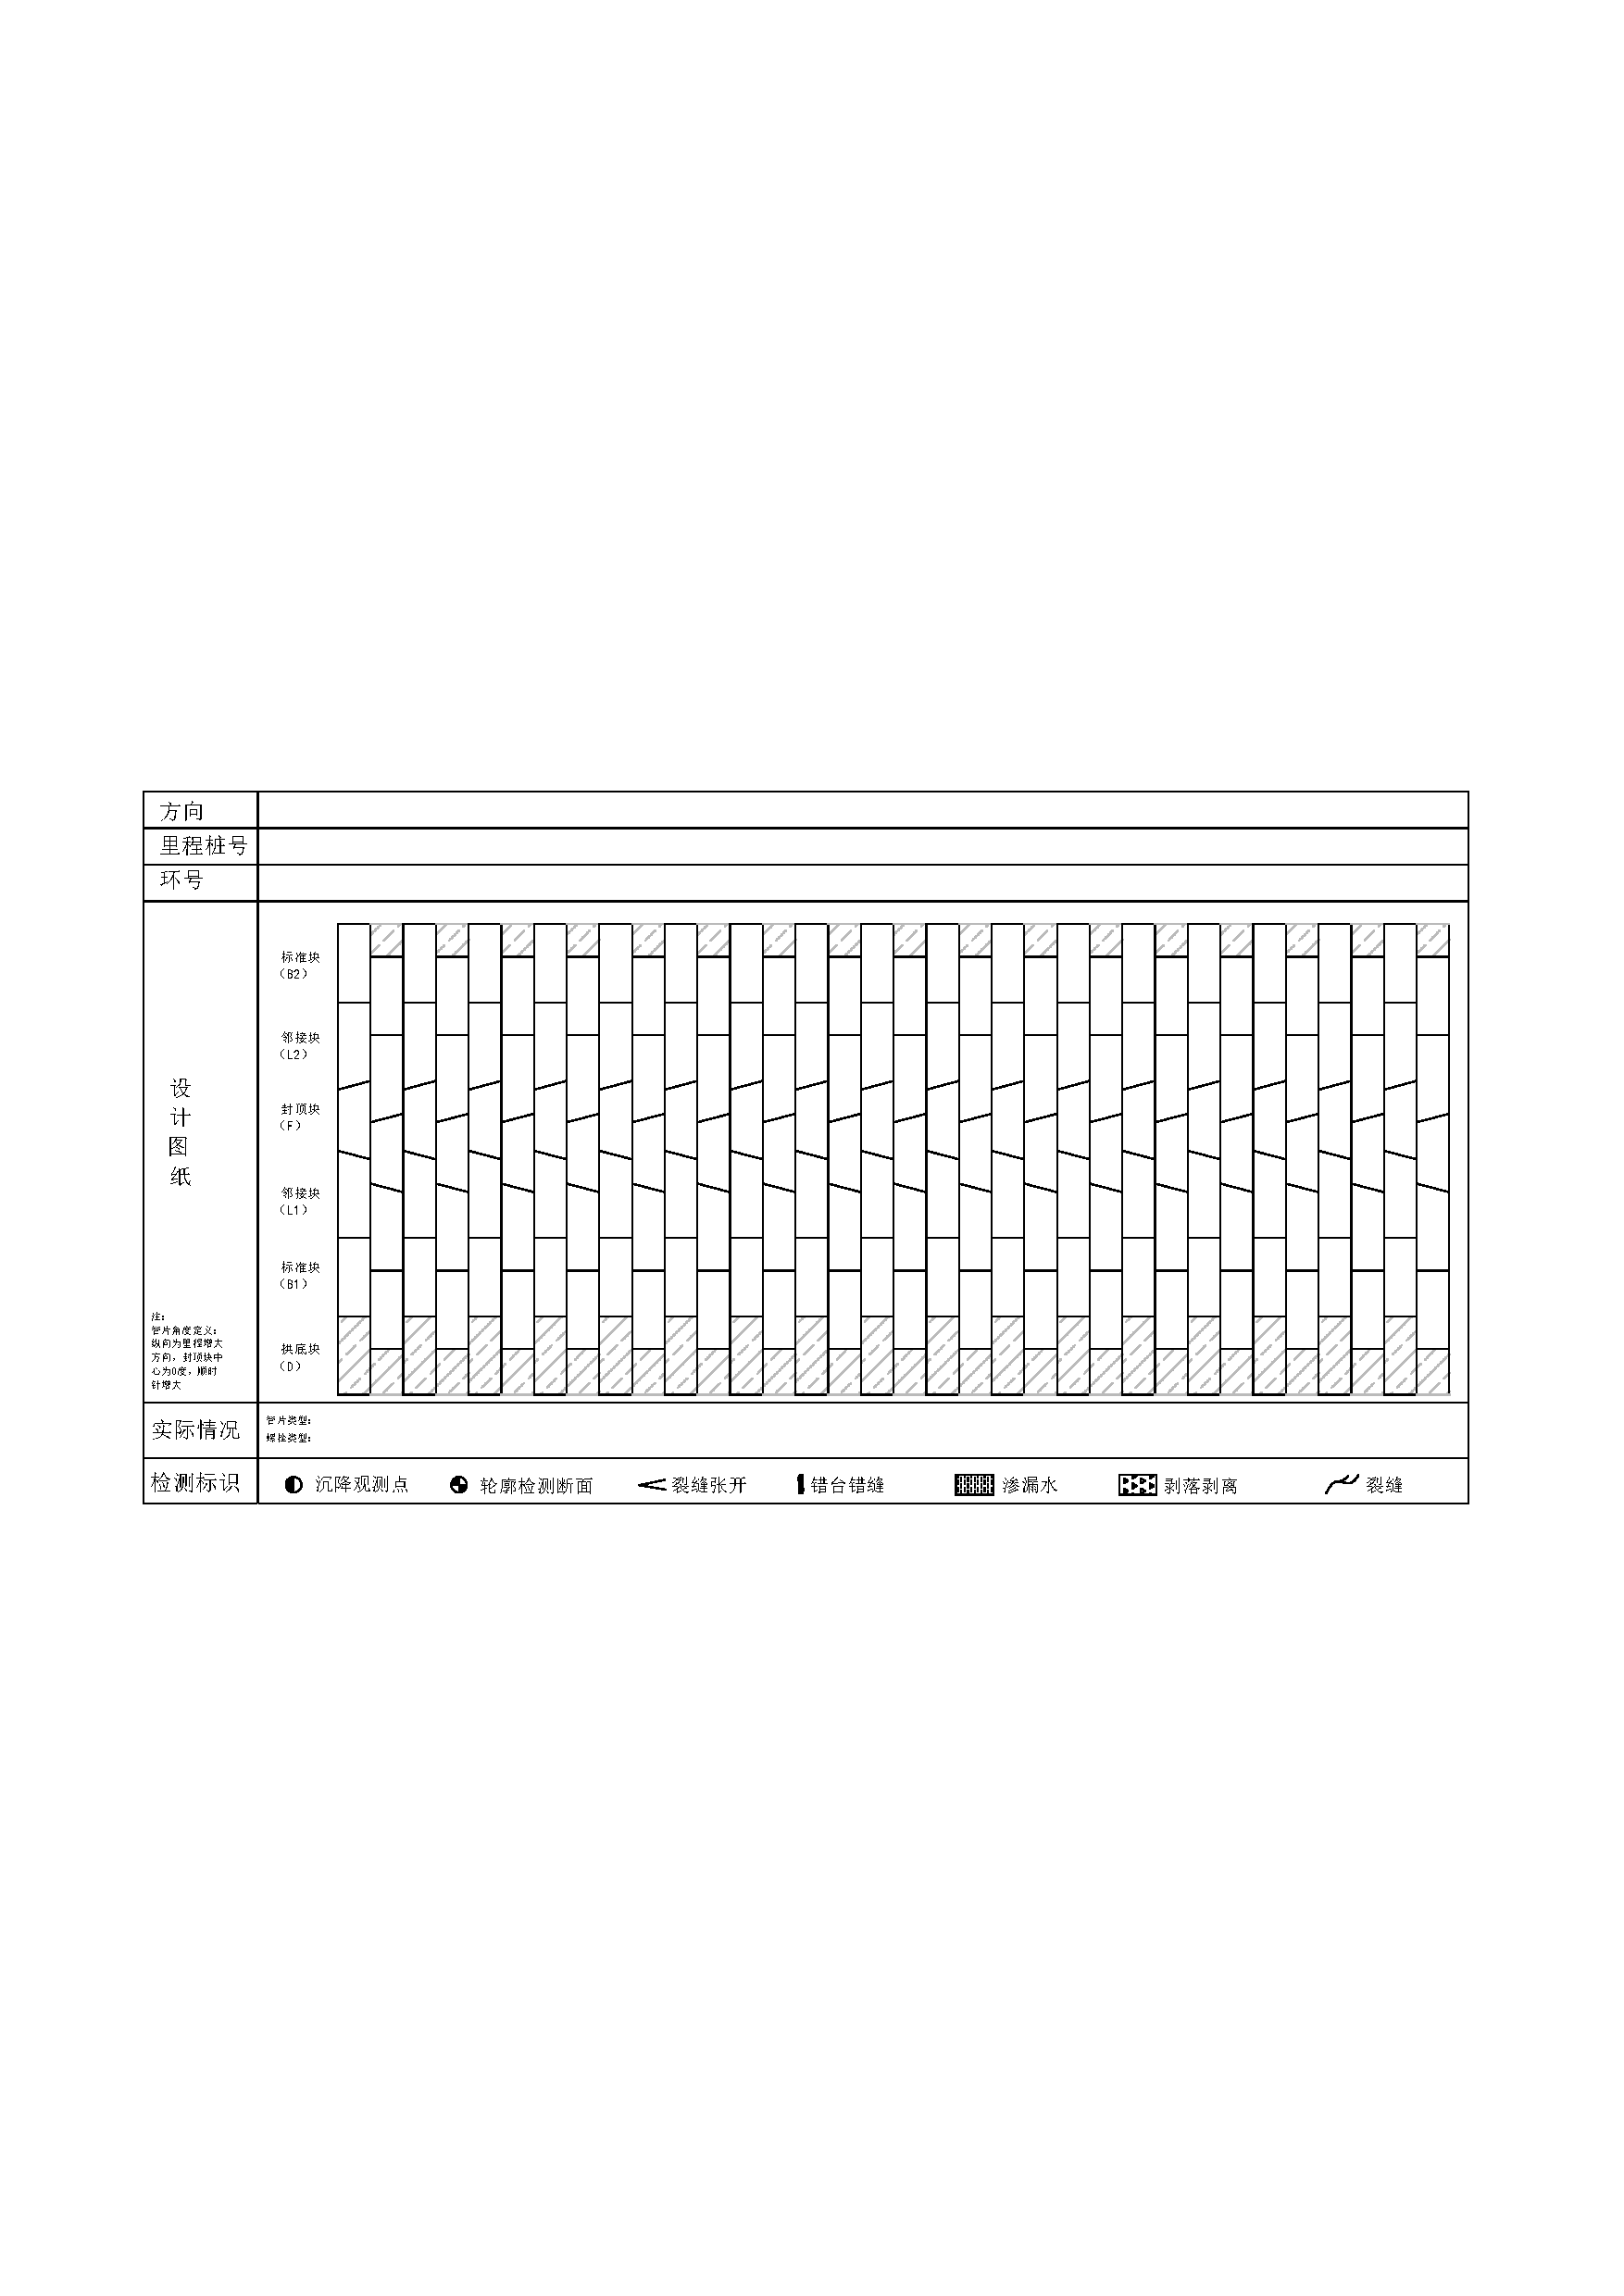
\includegraphics[width=1.0\textwidth]{chap2/distress-check.pdf}
    \caption{盾构隧道病害检查素描底图}
    \label{fig:盾构隧道病害检查素描底图}
\end{figure}

%%%%%%%%%%%%%%%%%%%%%%%%%%%%%%%%%%%%%%%%%%%%%%%%%%%%%%%%%%%%%%%%%%%
\section{盾构隧道服役性能评估指标}

根据上海地铁盾构隧道自身结构组成、内外部工作环境、日常监测、检测数据,以及盾构法隧道结构服役性能鉴定规范和公路和铁路交通隧道检查手册等规范规定,有许多参数可以作为服役性能评估的指标,笔者从已有的规范、研究(关宝树,\citeyear{关宝树1993日本铁路隧道维修养护管理技术的现状};FHWA,\citeyear{FHWA2005Highway};DG/TJ08-2123-2013,\citeyear{DGTJ0821232013};刘涛,\citeyear{刘涛2008既有盾构隧道结构性能评价研究};罗鑫,\citeyear{罗鑫2008公路隧道健康状态评估方法及系统研究};胥犇等,\citeyear{胥犇2010盾构隧道结构病害状态综合评价方法研究};腾丽,\citeyear{滕丽2012基于土体力学特性的盾构隧道施工风险监控系统研究};杨春山,\citeyear{杨春山2012运营地铁盾构隧道衬砌结构安全评估体系研究};朱宝林,\citeyear{朱宝林2014运营地铁盾构隧道状态评估及预测方法研究};陈楠,\citeyear{陈楠2017考虑发展趋势与指标关联的隧道结构健康评估方法研究};陈雪琴,\citeyear{陈雪琴2017交通基础设施服役性能评估和预测以及养护时机优化分析})收集整理了目前已有的评估指标,这些指标涵盖水文地质、设计、施工、材料、监测、检测等多个方面,包括拱顶水压力、地下水腐蚀性、承压水压力、土含水量、土渗透性、地表沉降、距工作井距离、距穿越段距离、隧道曲率半径、高程偏差、水平偏差、错台、注浆量、注浆压力、混凝土强度、渗透性、碳化深度、混凝土厚度、钢筋锈蚀、螺栓强度、锈蚀、止水条老化、垫层压缩量、累积沉降、差异沉降、沉降速率、渗漏水、裂缝、接缝张开、剥落、离子浓度、湿度、衬砌背后空洞等,并收集了各个指标分级的建议值(一般指标分级分为四级或者五级,本文整理时统一归为四级),如表~\ref{tab:盾构隧道评估指标与评估标准统计}~所示。

\begin{longtable}{?c"m{6.565em}"m{2.19em}"m{4em}"m{4.75em}"m{4.875em}"m{4em}?}
    \caption{盾构隧道评估指标与评估标准统计}
    \label{tab:盾构隧道评估指标与评估标准统计}\\
    \thickhline
    \multicolumn{1}{?m{3.25em}<{\centering}"}{分类} & \multicolumn{1}{c"}{评估指标}  & \multicolumn{1}{c"}{单位}    & \multicolumn{4}{m{17.625em}<{\centering}?}{评判标准(从好到差)} \bigstrut\\
    \thinhline
    \endfirsthead

    \caption{盾构隧道评估指标与评估标准统计(续表)}
    \label{tab:盾构隧道评估指标与评估标准统计}\\
    \thickhline
    \multicolumn{1}{?m{3.25em}<{\centering}"}{分类} & \multicolumn{1}{c"}{评估指标}  & \multicolumn{1}{c"}{单位}    & \multicolumn{4}{m{17.625em}<{\centering}?}{评判标准(从好到差)} \bigstrut\\
    \thinhline
    \endhead

    \thickhline
    \multicolumn{7}{r}{下页续表}
    \endfoot

    \thickhline
    \endlastfoot

    \multicolumn{1}{?c"}{\multirow{6}[12]{*}{地质}} & 拱顶水土压力 & 差比    & <0.08 & 0.08-0.15 & 0.15-0.23 & >0.23 \bigstrut\\
\cline{2-7}          & 地下水腐蚀性 & ph    & 6.1-7.9 & 5.1-6.0 & 4.1-5.0 & >4.0 \bigstrut\\
\cline{2-7}          & 承压水压力 & Mpa   & 0-0.1 & 0.1-0.2 & 0.2-0.4 & >0.4 \bigstrut\\
\cline{2-7}          & 土的含水量 & \%    & 0-65  & 65-70 & 70-80 & >80 \bigstrut\\
\cline{2-7}          & 土的渗透性 & \multicolumn{1}{c"}{} & \multicolumn{1}{c"}{} & \multicolumn{1}{c"}{} & \multicolumn{1}{c"}{} & \multicolumn{1}{c?}{} \bigstrut\\
\cline{2-7}          & 地表沉降  & mm    & 0-10  & \multicolumn{1}{c"}{10-30} & 30-50 & >50 \bigstrut\\
    \hline
    \multicolumn{1}{?c"}{\multirow{3}[6]{*}{设计}} & 距工作井距离 & \multicolumn{1}{c"}{} & \multicolumn{1}{c"}{} & \multicolumn{1}{c"}{} & \multicolumn{1}{c"}{} & \multicolumn{1}{c?}{} \bigstrut\\
\cline{2-7}          & 距穿越段距离 & \multicolumn{1}{c"}{} & \multicolumn{1}{c"}{} & \multicolumn{1}{c"}{} & \multicolumn{1}{c"}{} & \multicolumn{1}{c?}{} \bigstrut\\
\cline{2-7}          & 隧道曲率半径 & m     & >15000 & 5300-1500 & 1200-5300 & <1200 \bigstrut\\
    \hline
    \multicolumn{1}{?c"}{\multirow{6}[12]{*}{施工}} & 高程偏差  & mm    & <30   & 30-50 & 50-100 & >100 \bigstrut\\
\cline{2-7}          & 水平偏差  & mm    & <30   & 30-50 & 50-100 & >100 \bigstrut\\
\cline{2-7}          & 环向错台  & mm    & 0-5   & 5-8   & 8-12  & >12 \bigstrut\\
\cline{2-7}          & 径向错台  & mm    & 0-5   & 5-8   & 8-12  & >12 \bigstrut\\
\cline{2-7}          & 注浆量   & 差比    & <0.05 & 0.05-0.1 & 0.1-0.2 & >0.2 \bigstrut\\
\cline{2-7}          & 注浆压力  & 差比    & 0-0.1 & 0.1-0.2 & 0.2-0.4 & >0.4 \bigstrut\\
    \hline
    \multicolumn{1}{?c"}{\multirow{10}[20]{*}{材料}} & 混凝土强度 & 差比    & 0-0.1 & 0.1-0.33 & 0.33-0.5 & >0.5 \bigstrut\\
\cline{2-7}          & 混凝土渗透性 & \multicolumn{1}{c"}{} & \multicolumn{1}{c"}{} & \multicolumn{1}{c"}{} & \multicolumn{1}{c"}{} & \multicolumn{1}{c?}{} \bigstrut\\
\cline{2-7}          & 混凝土碳化 & \multicolumn{1}{c"}{} & \multicolumn{1}{c"}{} & \multicolumn{1}{c"}{} & \multicolumn{1}{c"}{} & \multicolumn{1}{c?}{} \bigstrut\\
\cline{2-7}          & 混凝土厚度 & 差比    & 0-0.1 & 0.1-0.33 & 0.33-0.5 & >0.5 \bigstrut\\
\cline{2-7}          & 钢筋锈蚀  & \multicolumn{1}{c"}{} & 没有锈蚀  & 斑点腐蚀,局部薄层锈蚀生成物 & 薄层锈蚀生成物,混凝土表面粘附锈生成物 & 明显膨胀性锈蚀生成物,断面出现缩减 \bigstrut\\
\cline{2-7}          & 螺栓强度  & \multicolumn{1}{c"}{} & \multicolumn{1}{c"}{} & \multicolumn{1}{c"}{} & \multicolumn{1}{c"}{} & \multicolumn{1}{c?}{} \bigstrut\\
\cline{2-7}          & 螺栓锈蚀  & \multicolumn{1}{c"}{} & \multicolumn{1}{c"}{} & \multicolumn{1}{c"}{} & \multicolumn{1}{c"}{} & \multicolumn{1}{c?}{} \bigstrut\\
\cline{2-7}          & 螺栓松动  & \multicolumn{1}{c"}{} & \multicolumn{1}{c"}{} & \multicolumn{1}{c"}{} & \multicolumn{1}{c"}{} & \multicolumn{1}{c?}{} \bigstrut\\
\cline{2-7}          & 止水条老化 & \multicolumn{1}{c"}{} & \multicolumn{1}{c"}{} & \multicolumn{1}{c"}{} & \multicolumn{1}{c"}{} & \multicolumn{1}{c?}{} \bigstrut\\
\cline{2-7}          & 垫层压缩量 & mm    & 0-1   & 1-3   & 3-5   & >5 \bigstrut\\
    \hline
    \multicolumn{1}{?c"}{\multirow{13}[26]{*}{监测}} & 累计沉降  & mm    & 0-60  & 60-120 & 120-160 & >160 \bigstrut\\
\cline{2-7}          & 差异沉降  & mm /100m & 0-20  & 20-40 & 40-60 & >60 \bigstrut\\
\cline{2-7}          & 沉降速度  & \multicolumn{1}{c"}{} & \multicolumn{1}{c"}{} & \multicolumn{1}{c"}{} & \multicolumn{1}{c"}{} & \multicolumn{1}{c?}{} \bigstrut\\
\cline{2-7}          & 直径椭圆度 & ‰D    & 0-1   & 1-3   & 3-5   & >5 \bigstrut\\
\cline{2-7}          & 收敛速度  & mm /年  & 0-1   & 1-3   & 3-10  & >10 \bigstrut\\
\cline{2-7}          & 渗漏水   & \multicolumn{1}{c"}{} & 渗润    & 滴水    & 流水    & 喷水 \bigstrut\\
\cline{2-7}          & 裂缝长度  & m     & 0-2   & \multicolumn{1}{l"}{2-5} & \multicolumn{1}{l"}{5-10} & >10 \bigstrut\\
\cline{2-7}          & 裂缝宽度  & mm    & 0-0.2 & 0.2-0.3 & 0.3-0.5 & >0.5 \bigstrut\\
\cline{2-7}          & 接缝张开  & mm    & 0-0.2 & 0.2-1 & \multicolumn{1}{c"}{1-6} & >6 \bigstrut\\
\cline{2-7}          & 破损剥落  & \multicolumn{1}{c"}{} & \multicolumn{1}{c"}{} & \multicolumn{1}{c"}{} & \multicolumn{1}{c"}{} & \multicolumn{1}{c?}{} \bigstrut\\
\cline{2-7}          & 氯离子浓度 & \multicolumn{1}{c"}{} & \multicolumn{1}{c"}{} & \multicolumn{1}{c"}{} & \multicolumn{1}{c"}{} & \multicolumn{1}{c?}{} \bigstrut\\
\cline{2-7}          & 湿度    & \multicolumn{1}{c"}{} & \multicolumn{1}{c"}{} & \multicolumn{1}{c"}{} & \multicolumn{1}{c"}{} & \multicolumn{1}{c?}{} \bigstrut\\
\cline{2-7}          & 衬砌背后空洞 & mm    & 0-100 & 100-200 & 200-500 & 500-1000 \bigstrut\\
\end{longtable}

诚然上述指标均能在一定程度反映盾构隧道服役性能,但是选择所有的指标并不符合实际情况,体现在(1)土体含水量、环境中的离子浓度等不在日常检查范围内,一般情况下缺失此类数据;(2)监测隧道周围水土压力、结构内力等的传感器寿命有限,损坏率高,且损坏后维修更换不便,这些指标在隧道全寿命周期的获取不可靠;(3)混凝土碳化深度、钢筋锈蚀程度、止水带老化等由于检查难度较大,成本较高,且有可能检测会破坏隧道本身结构,故也不推荐选取此类指标。综上所述,结合上海地铁盾构隧道病害检查实际情况,本文将考虑选取沉降、收敛、衬砌渗漏水、裂缝、剥落、接缝张开、错台等作为评估指标,这些指标可以分为三大类:纵向变形、横向变形和衬砌病害指标。

%+++++++++++++++++++++++++++++++++++++++++++++++++++++++++++++++++%
\subsection{纵向变形}

\subsubsection{累积沉降}

根据现场监测数据显示,上海地铁盾构隧道在竣工后超过10年的营运期间,产生较大的结构沉降和不均匀沉降,沉降速率在竣工后一段时间较大,后期逐渐减少(Shen等,\citeyear{shen2014long})。导致沉降量大的原因有许多,最主要的是上海地区整体大地沉降,根据记录,上海市中心的大地沉降大2-3m(Chai等,\citeyear{chai2004land}),这是大量抽取地下水以及城市化过程的外荷载等因素导致,如地铁附近工程建设、地铁线路穿越、地表循环荷载等。

\begin{figure}[htbp]
    \centering
    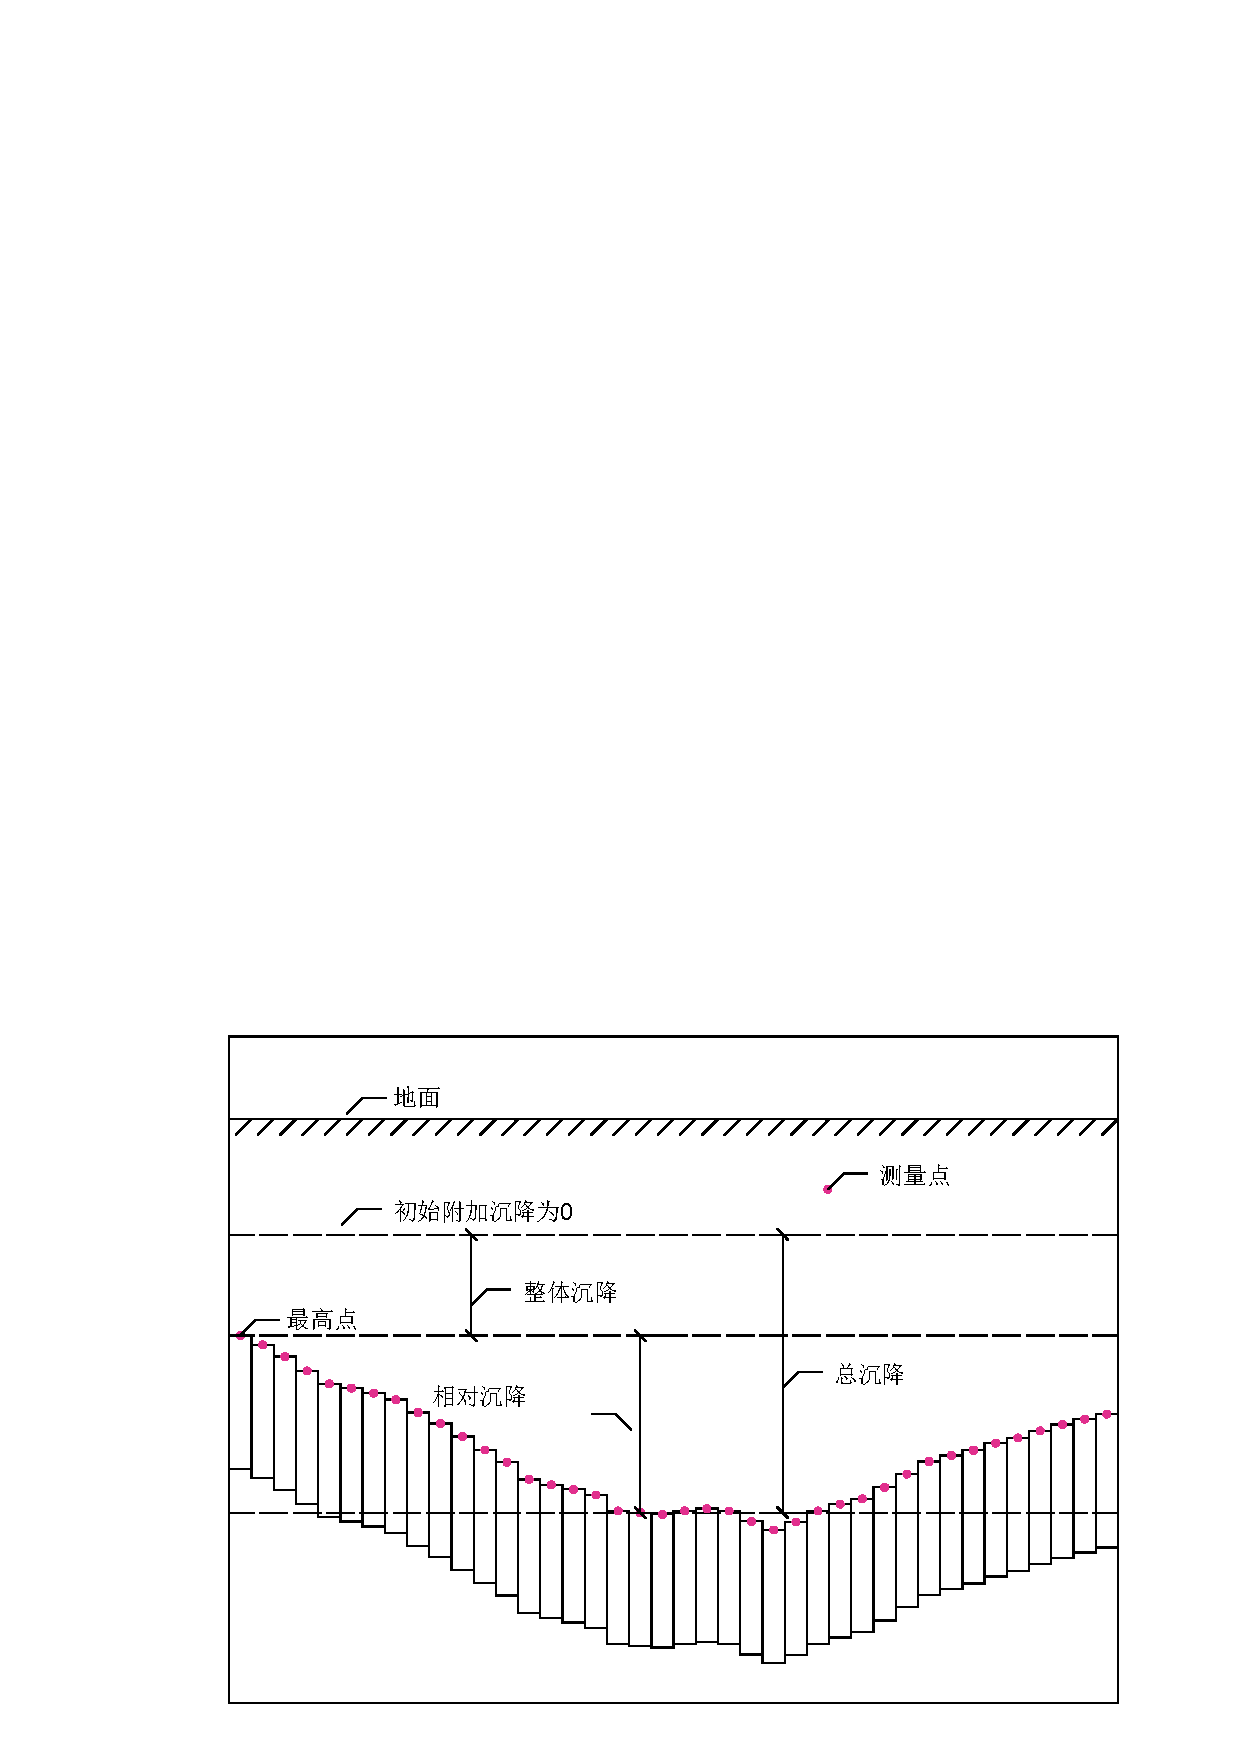
\includegraphics[width=0.8\textwidth]{chap2/relative-sett.pdf}
    \caption{隧道相对沉降示意图}
    \label{fig:隧道相对沉降示意图}
\end{figure}

隧道的累积沉降是反映隧道服役性能的重要指标。因为隧道本身处于土体介质中,大地沉降导致的隧道整体沉降对结构安全危害较小。为排除大地沉降因素的影响,本文采用相对沉降的概念,如图~\ref{fig:隧道相对沉降示意图}~所示。假设隧道建成时的初始附加沉降为0,经过若干运营时间后,将附加沉降最小的衬砌环定义为最高点,假设最高点的附加沉降即为大地整体沉降,相对沉降则为总沉降减去整体沉降。累积相对沉降的计算公式为
\begin{align}
    \label{equ:sett_r}
    {sett}_{ri}={sett}_{ti}-{sett}_{u} \\
    \label{equ:sett_ave}
    {sett}_{a}=\frac{\sum\limits_{i=1}^{n}{{sett}_{ri}}}{n}
\end{align}
式中:${sett}_{ri}$为第$i$个监测点相对沉降;${sett}_{ti}$为第$i$个监测点总沉降;${sett}_{u}$为大地整体沉降;${sett}_{a}$为相对沉降平均值;$n$为隧道监测点数量。

\subsubsection{差异沉降}

Shen等(\citeyear{shen2014long})提出差异沉降也是影响隧道服役性能的重要指标,总结了上海地铁隧道差异沉降的主要原因:(1)隧道下卧地层条件差异;(2)地铁车站与隧道之间刚度不同导致的差异沉降;(3)联络通过与隧道刚度不一致;(4)隧道下穿河流易导致差异沉降。在实际工程中,差异沉降一般采用曲率半径表示,如王如路和刘建航(\citeyear{王如路2004上海地铁监护实践})指出曲率半径可采用布置在地铁区间隧道内(道床或管片上)监测点的测量数据,按经验计算公式计算
\begin{equation}
    \label{equ:ratio1}
    \rho =\frac{{{(L/4)}^{2}}}{{{\delta }_{m}}}
\end{equation}
式中:$\rho$为最小曲率半径;$L$为沉降范围,取区间隧道长度;${\delta }_{m}$为沉降最大值。也有取计算点临近的三点沉降监测点,由三点确定一圆弧,近似取圆弧曲率半径的计算方法。叶耀东(\citeyear{叶耀东2007软土地区运营地铁盾构隧道结构变形及健康诊断方法研究})则提出采用三次B样条曲线模拟整条隧道变形再计算曲率半径的方法。

采用曲率半径表示差异沉降只是一种近似的计算方法,而且不一定能计算得到每一监测点处的差异沉降。故本文直接采用差异沉降定义的计算方法
\begin{align}
    \label{equ:diff_sett}
    set{{t}_{d\_i}}=\frac{\left| set{{t}_{ri}}-set{{t}_{r(i-1)}} \right|}{{{l}_{i}}} \\
    \label{equ:diff_sett_ave}
    set{{t}_{d\_ave}}=\frac{\sum\limits_{i=2}^{n}{set{{t}_{d\_i}}}}{n-1}
\end{align}
式中:$set{{t}_{d\_i}}$为第$i$个监测点与第$i-1$个监测点的差异沉降;$set{{t}_{ri}}$为第$i$个监测点相对沉降;$set{{t}_{r(i-1)}}$为第$i-1$个监测点相对沉降;${l}_{i}$为第$i$个监测点与第$i-1$个监测点的距离;$set{{t}_{d\_a}}$为平均差异沉降值;$n$为隧道监测点数量。

%+++++++++++++++++++++++++++++++++++++++++++++++++++++++++++++++++%
\subsection{横向变形}

上海地铁设计时要求横向累积变形量小于$5\%D$($D$为隧道外直径),但在实际监测中发现,运营隧道的收敛变形往往超过此限定值,过大的横向变形会引起衬砌接缝张开和挤压、渗漏水或管片压损等(Mahdevari和Torabi,\citeyear{mahdevari2012prediction})。本文采用平均收敛变形率表征隧道横向变形的程度
\begin{equation}
    \label{equ:conv_ave}
    {{cov}_{a}}=\frac{\sum\limits_{i=1}^{m}{\left| {{d}_{i}}-D \right|}}{Dm}
\end{equation}
式中:${cov}_{a}$为平均收敛变形率;${d}_{i}$为第$i$个收敛监测点外直径;$D$为隧道外直径设计值;$m$为收敛监测点数。

%+++++++++++++++++++++++++++++++++++++++++++++++++++++++++++++++++%
\subsection{衬砌病害}

上海地铁人工检查病害包括渗漏水、裂缝、剥落、接缝张开和错台。图~\ref{fig:上海地铁病害统计图}~展示了地铁1号线、2号线、4号线在2011年和2012年的病害数量统计,其中渗漏水总计3544处记录,占病害总数73.6\%,裂缝总计696处记录,占病害总数14.5\%,剥落548处记录,占病害总数11.4\%。从图中可看出,接缝张开与错台在实际检查数据占的比例非常小,主要原因是这两个病害一般数值较小,在肉眼检查时较难观察到。

\begin{figure}[htbp]
    \centering
    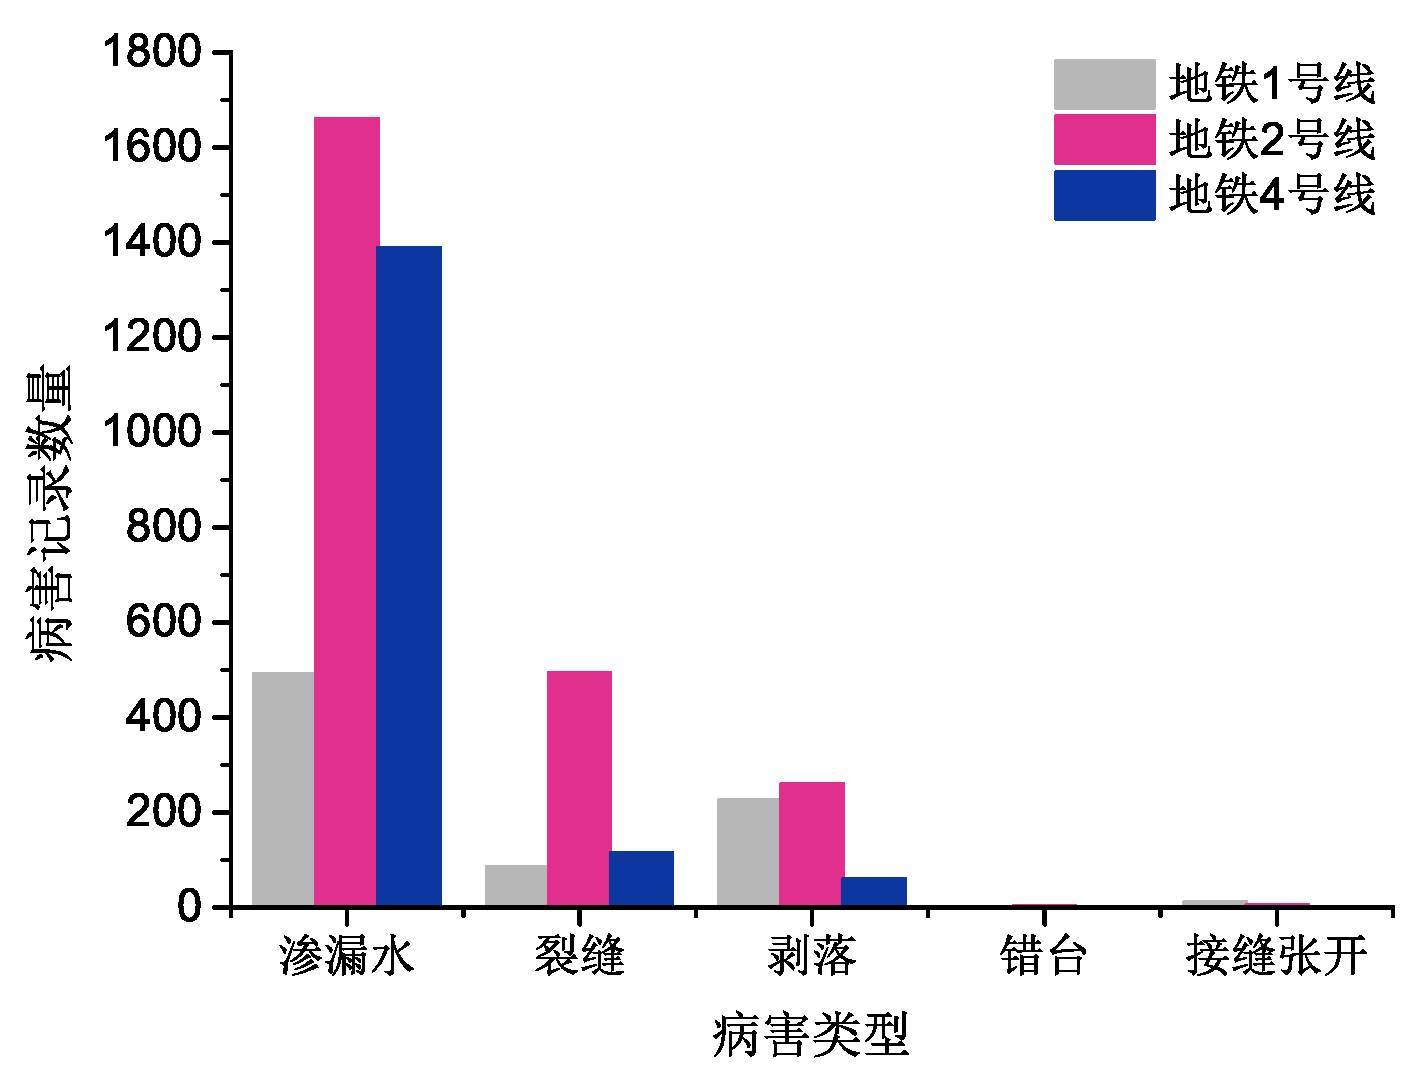
\includegraphics[width=0.8\textwidth]{chap2/distress-num.eps}
    \caption{上海地铁病害统计图}
    \label{fig:上海地铁病害统计图}
\end{figure}

另一方面,许多学者研究得出接缝张开和错台与隧道的沉降和收敛有较大相关性。王如路和张冬梅(\citeyear{王如路2013超载作用下软土盾构隧道横向变形机理及控制指标研究})根据隧道衬砌管片之间的相对位置,仅考虑管片在横向收敛时只发生相对转动和平动,采用几何学方法,得出接缝张开与横向收敛的关系,如图~\ref{fig:衬砌管片横向收敛与接缝张开几何关系图}~所示。

\begin{figure}[htbp]
    \centering
    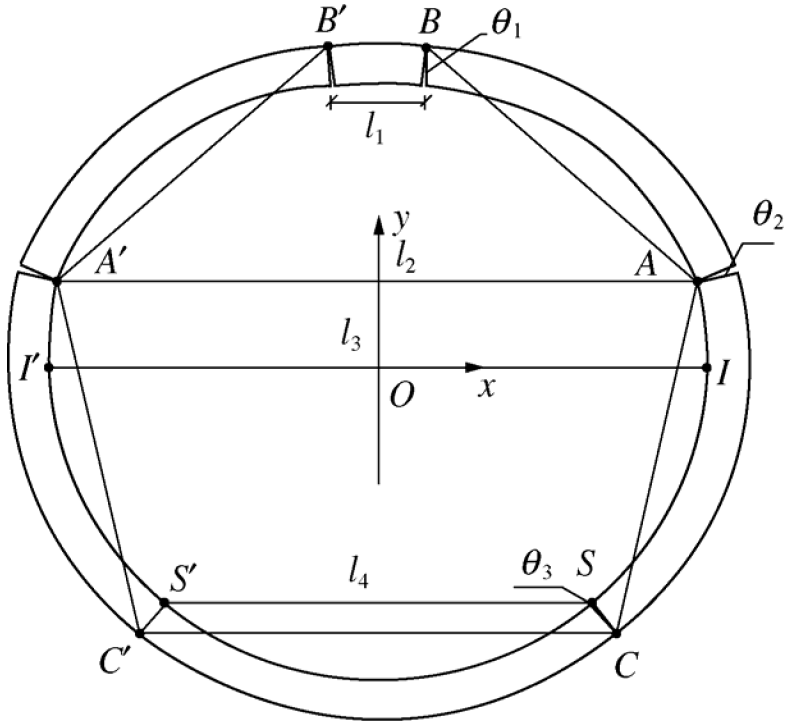
\includegraphics[width=0.5\textwidth]{chap2/lining-geom.png}
    \caption{衬砌管片横向收敛与接缝张开几何关系图}
    \label{fig:衬砌管片横向收敛与接缝张开几何关系图}
\end{figure}

廖少明等(\citeyear{廖少明2005隧道纵向剪切传递效应及其一维解析})根据弹性地基梁理论,提出隧道纵向剪切传递的概念,如图~\ref{fig:弹性地基梁纵向剪切平衡分析图}~所示。认为隧道的纵向不均匀沉降将导致隧道纵向变形剪切,也即是错台病害的产生。

\begin{figure}[htbp]
    \centering
    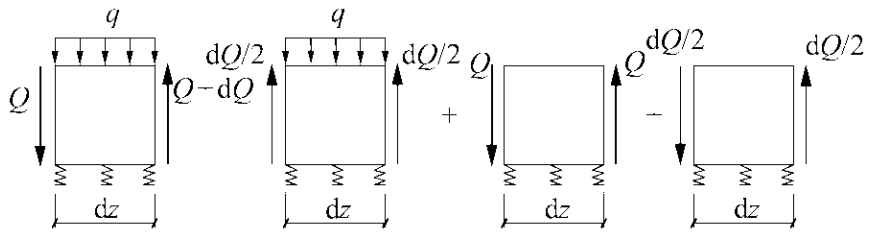
\includegraphics[width=0.9\textwidth]{chap2/sett-shear.png}
    \caption{弹性地基梁纵向剪切平衡分析图}
    \label{fig:弹性地基梁纵向剪切平衡分析图}
\end{figure}

因此,本文只选取渗漏水、裂缝、剥落作为评估指标,如式~\ref{equ:leakage}~-~\ref{equ:cracking}~所示,其中:$r$为检查隧道区间总环数;${d}_{l}$为百环渗漏水面积($m^2/100$环);${d}_{s}$为百环衬砌剥落面积($m^2/100$环);${d}_{c}$为百环裂缝长度($m/100$环);${n}_{l}$为渗漏水记录总数;${n}_{s}$为剥落记录总数;${n}_{c}$为裂缝记录总数;${l}_{ai}$为第$i$个渗漏水面积;${s}_{ai}$为第$i$个剥落面积;${c}_{li}$为第$i$个裂缝长度。
\begin{align}
    \label{equ:leakage}
    {{d}_{l}}=\frac{\sum\limits_{i=1}^{{{n}_{l}}}{{{l}_{ai}}}}{r}\times 100 \\
    \label{equ:spalling}
    {{d}_{s}}=\frac{\sum\limits_{i=1}^{{{n}_{s}}}{{{s}_{ai}}}}{r}\times 100 \\
    \label{equ:cracking}
    {{d}_{c}}=\frac{\sum\limits_{i=1}^{{{n}_{c}}}{{{c}_{li}}}}{r}\times 100
\end{align}
%+++++++++++++++++++++++++++++++++++++++++++++++++++++++++++++++++%
\subsection{指标特征}

综上所述,本文选取了六个观测变量:相对沉降平均值${sett}_{a}$、平均差异沉降$set{{t}_{d\_a}}$、平均收敛变形率${cov}_{a}$、百环渗漏水面积${d}_{l}$、百环衬砌剥落面积${d}_{s}$、百环裂缝长度${d}_{c}$作为评估指标。表~\ref{tab:上海地铁观测变量统计信息}~统计了上海地铁盾构隧道上述六个观测变量的相关信息,后续的评估结果可用于与此类似的盾构隧道工程。

\begin{table}[htbp]
  \centering
  \caption{上海地铁观测变量统计信息}
    \begin{tabular}{?m{5em}<{\centering}"c"c"c"c"c"c?}
    \thickhline
    观测变量  & 最小值   & 第一四分位 & 中位数   & 第三四分位 & 最大值   & 平均值 \bigstrut\\
    \thinhline
    ${sett}_{a}$\newline($mm$)  & 1.2   & 8.2   & 19.6  & 40.2  & 130.1  & 27.8  \bigstrut\\
    \thinhline
    $set{{t}_{d\_a}}$\newline($mm/100m$) & 1.5   & 4.2   & 9.5   & 19.8  & 58.0  & 12.5  \bigstrut\\
    \thinhline
    ${cov}_{a}$\newline($‰D$)  & 2.4   & 6.1   & 7.3   & 8.4   & 12.0  & 1.5  \bigstrut\\
    \thinhline
    ${d}_{l}$\newline($m^2/100$环) & 0.00  & 0.16  & 0.42  & 1.11  & 5.74  & 0.86  \bigstrut\\
    \thinhline
    ${d}_{s}$\newline($m^2/100$环) & 0.00  & 0.00  & 0.00  & 0.90  & 5.67  & 0.76  \bigstrut\\
    \thinhline
    ${d}_{c}$\newline($m/100$环) & 0.00  & 0.00  & 0.00  & 0.01  & 1.30  & 0.08  \bigstrut\\
    \thickhline
    \end{tabular}%
  \label{tab:上海地铁观测变量统计信息}%
\end{table}%

%%%%%%%%%%%%%%%%%%%%%%%%%%%%%%%%%%%%%%%%%%%%%%%%%%%%%%%%%%%%%%%%%%%
\section{盾构隧道服役性能评估方法}

%+++++++++++++++++++++++++++++++++++++++++++++++++++++++++++++++++%
\subsection{专家评分}

隧道服役性能评分(TSR)通过专家打分表获取,没有采用现场巡查打分的原因是地铁隧道只有在地铁停运后,凌晨的4、5个小时才能进入,现场巡查的方式并不切合实际。图~\ref{fig:隧道服役性能评分表}~所示为TSR专家打分表,选取200环衬砌作为一次评估单位,因为评估长度选择太短,区间包含的病害较少,长度太长则不能保证隧道服役性能在区间保持不变。评分表上包含了样本的基本信息,包括地铁线路、起始终止车站、起始终止环号、病害检查日期,评分表上还包含了病害的位置、大小、形状,和沉降、收敛的监测数据。Yuan等(\citeyear{Yuan2012Assessment})和盾构法隧道结构服役性能鉴定规范(\citeyear{DGTJ0821232013})将隧道服役性能等级分为正常、退化、劣化、恶化、危险五个等级,本文参考此分级方法,将隧道服役性能等级分为5个级别,分别为很好(5分)、好(4分)、一般(3分)、差(2分)、很差(1分)。

\begin{figure}[htbp]
    \centering
    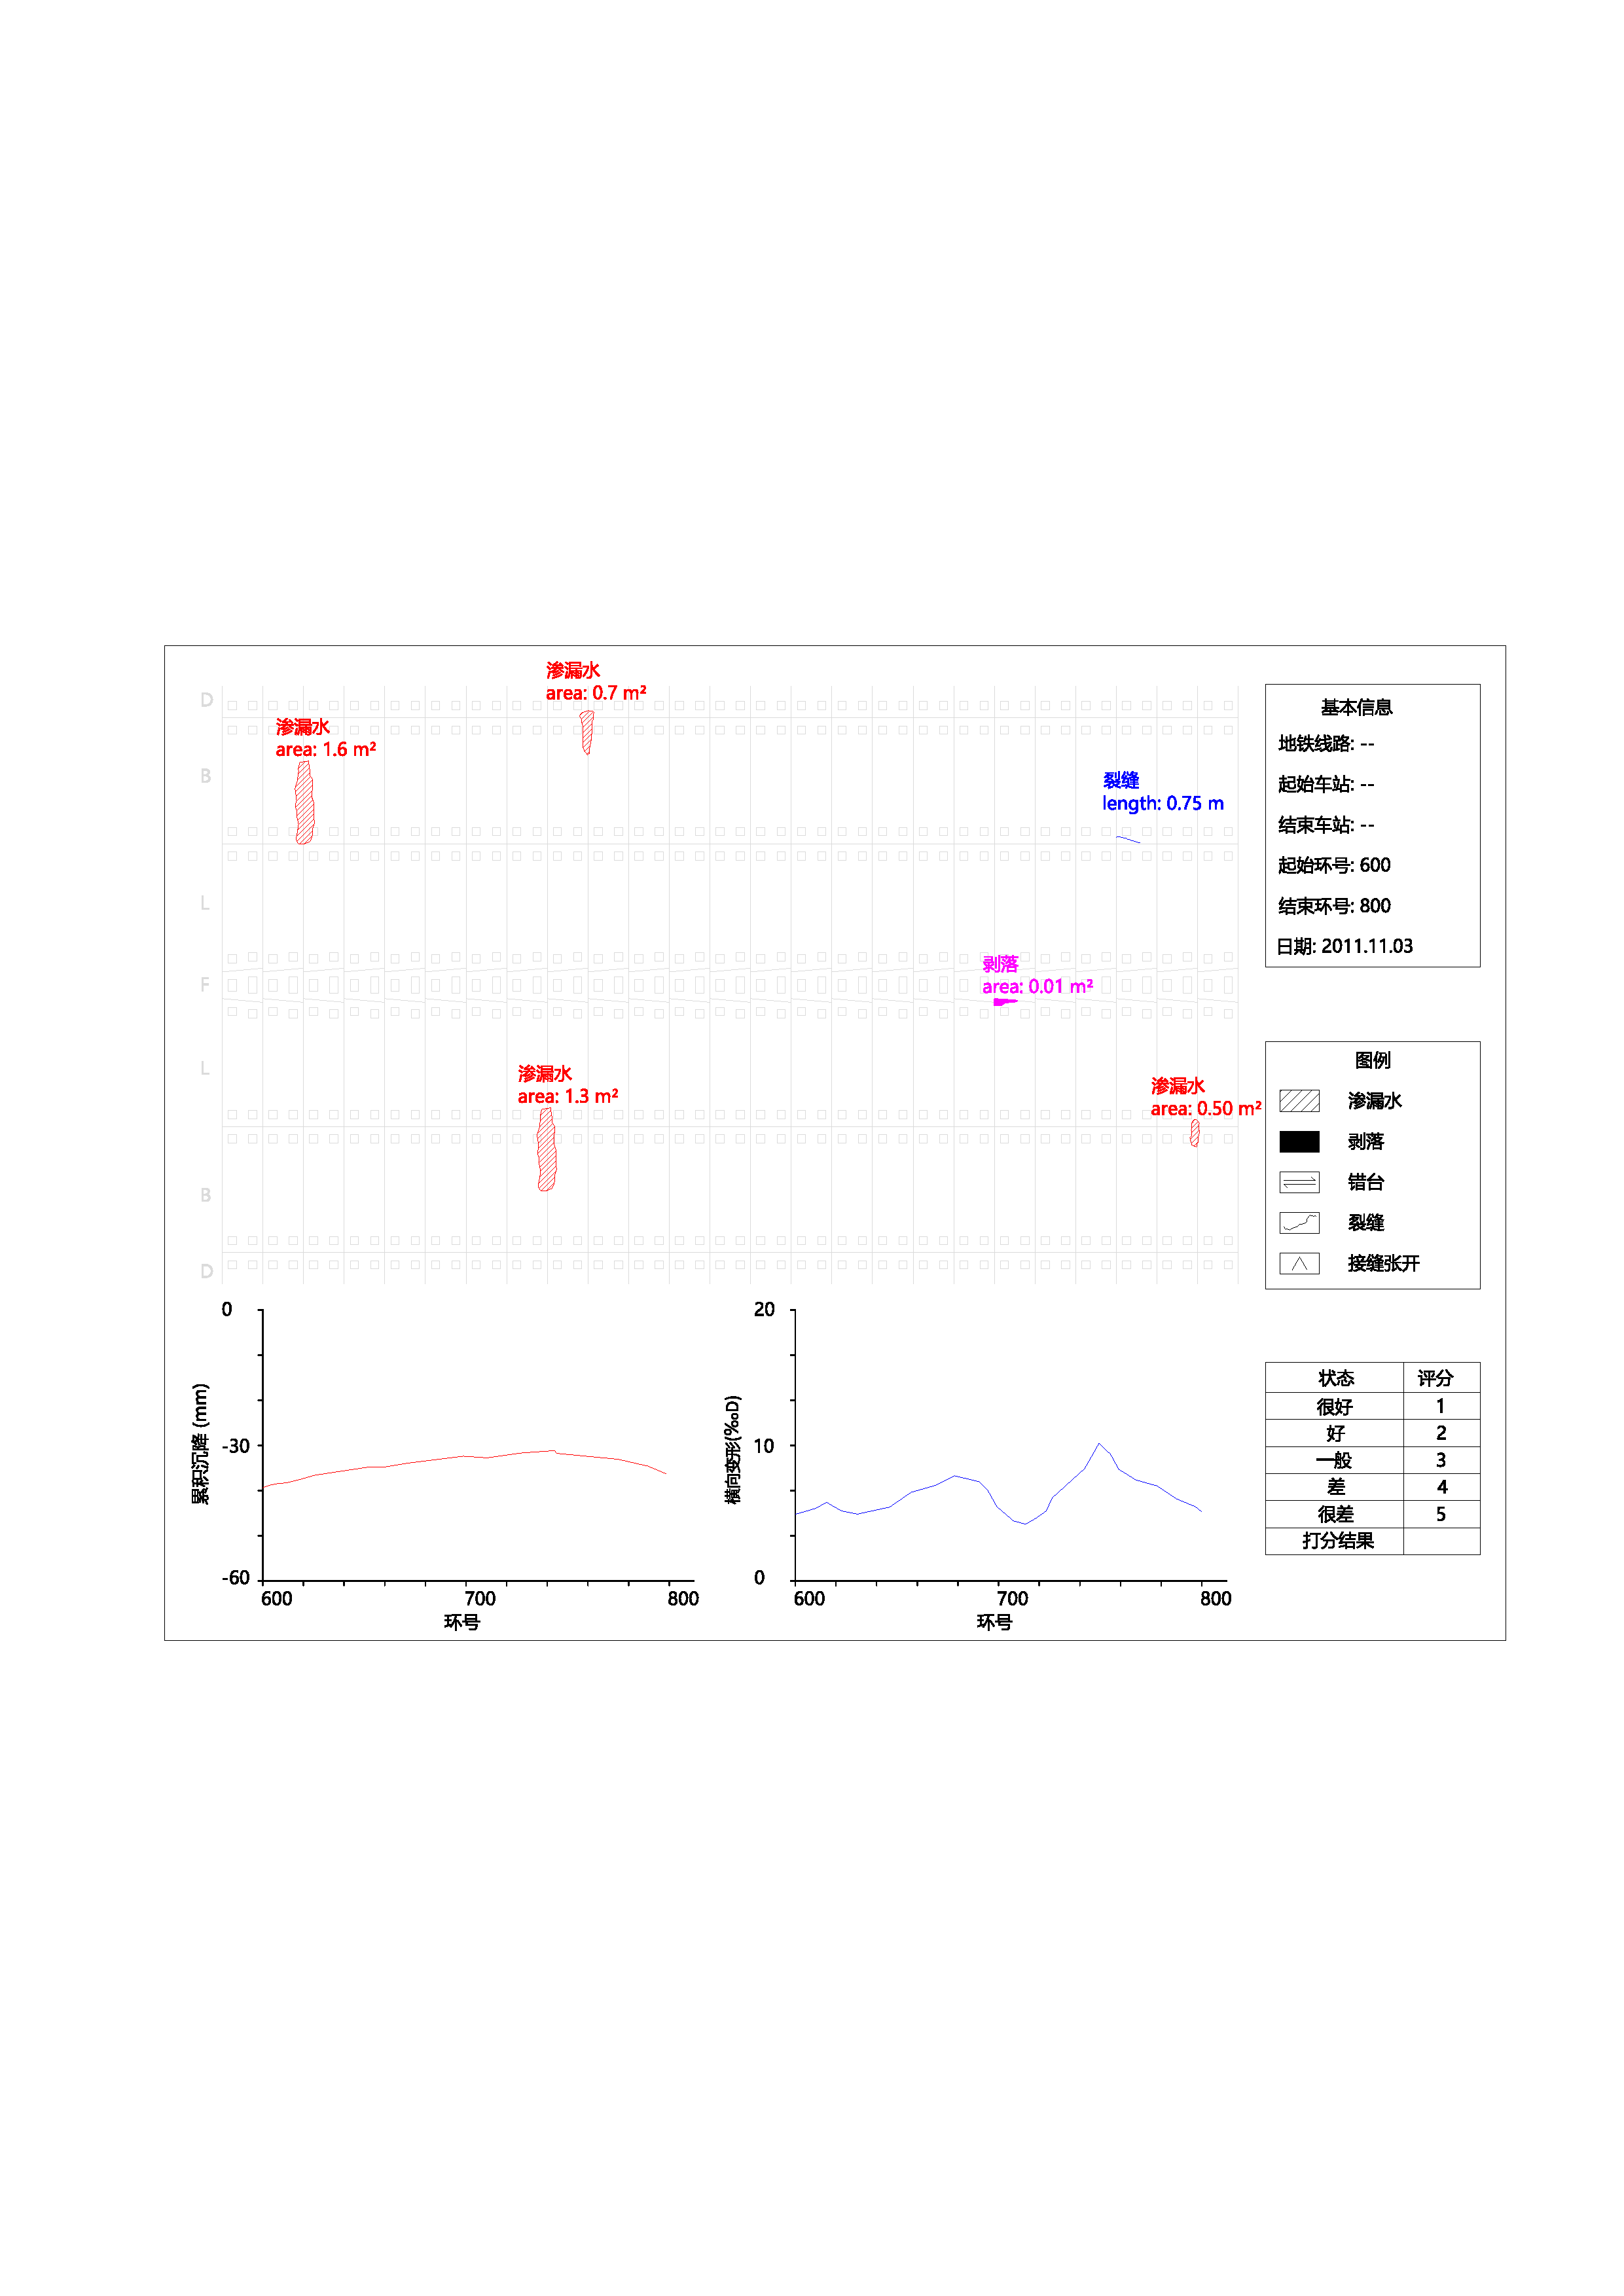
\includegraphics[width=1.0\textwidth]{chap2/tsr.pdf}
    \caption{隧道服役性能评分表}
    \label{fig:隧道服役性能评分表}
\end{figure}

\begin{table}[!htbp]
  \centering
  \caption{专家评分小组成员}
    \begin{tabular}{?m{5em}<{\centering}"m{5em}<{\centering}"m{5em}<{\centering}"m{8em}<{\centering}?}
    \thickhline
    序号    & 年龄    & 工作年限  & 背景 \bigstrut\\
    \thinhline
    1     & 45    & 14    & 地铁结构设计 \bigstrut\\
    \thinhline
    2     & 44    & 21    & 地铁施工 \bigstrut\\
    \thinhline
    3     & 60    & 36    & 结构监测 \bigstrut\\
    \thinhline
    4     & 43    & 9     & 结构养护 \bigstrut\\
    \thinhline
    5     & 41    & 10    & 结构养护 \bigstrut\\
    \thinhline
    6     & 36    & 10    & 结构维护 \bigstrut\\
    \thinhline
    7     & 47    & 27    & 结构维护 \bigstrut\\
    \thinhline
    8     & 40    & 10    & 结构研究 \bigstrut\\
    \thinhline
    9     & 46    & 17    & 岩土研究 \bigstrut\\
    \thickhline
    \end{tabular}%
  \label{tab:专家评分小组成员}%
\end{table}%

评分小组由9位专家组成,分别来自设计、施工、管理、维养和研究等背景的专家,如表~\ref{tab:专家评分小组成员}~所示。在评分前,会跟专家说明隧道服役性能的基本定义和假设,且允许专家一起讨论交流各自的意见,但在评分过程中专家禁止任何交流,直到完成评分为止。该评分小组于2015年1月17日对18个样本区间进行评分,于2015年5月23日对另外21个样本区间进行评分,评分结果如表~\ref{tab:隧道服役性能评分结果}~所示,其中第40个样本是假设隧道在初始状态没有任何病害、变形,其$TSR$应为5.0,表~\ref{tab:隧道服役性能评分结果}~第2列为样本所有评分的平均值,评分范围从4.9-2.1分,第3列为样本评分的标准差,第4到8列为样本的观测变量。


\begin{longtable}{?c"c"c"c"c"c"c"c"c?}
    \caption{隧道服役性能评分结果}
    \label{tab:隧道服役性能评分结果}\\
    \thickhline
    \multirow{3}[2]{*}{序号} & \multirow{3}[2]{2.85em}{TSR} & \multirow{3}[2]{3em}{TSR\newline 标准差} & \multirow{3}[2]{2.5em}{${sett}_{a}$\newline ($mm$)} & \multirow{3}[2]{4em}{$set{{t}_{d\_a}}$\newline ($mm/$\newline 100m)} & \multirow{3}[2]{2.5em}{${cov}_{a}$\newline ($‰D$)} & \multirow{3}[2]{3.5em}{${d}_{l}$\newline ($m^2/$\newline 百环)} & \multirow{3}[2]{3.5em}{${d}_{s}$\newline ($m^2/$\newline 百环)} & \multirow{3}[2]{3.5em}{${d}_{c}$\newline($m/$\newline 百环)} \bigstrut[t]\\
          &       &       &       &       &       &       &       &  \bigstrut[b]\\
         &       &       &       &       &       &       &       &  \bigstrut[b]\\          
    \thinhline
    \endfirsthead

    \caption{隧道服役性能评分结果(续表)}
    \label{tab:隧道服役性能评分结果}\\
    \thickhline
    \multirow{3}[2]{*}{序号} & \multirow{3}[2]{2.85em}{TSR} & \multirow{3}[2]{3em}{TSR\newline 标准差} & \multirow{3}[2]{2.5em}{${sett}_{a}$\newline ($mm$)} & \multirow{3}[2]{4em}{$set{{t}_{d\_a}}$\newline ($mm/$\newline 100m)} & \multirow{3}[2]{2.5em}{${cov}_{a}$\newline ($‰D$)} & \multirow{3}[2]{3.5em}{${d}_{l}$\newline ($m^2/$\newline 百环)} & \multirow{3}[2]{3.5em}{${d}_{s}$\newline ($m^2/$\newline 百环)} & \multirow{3}[2]{3.5em}{${d}_{c}$\newline($m/$\newline 百环)} \bigstrut[t]\\
          &       &       &       &       &       &       &       &  \bigstrut[b]\\
         &       &       &       &       &       &       &       &  \bigstrut[b]\\ 
    \thinhline
    \endhead

    \thickhline
    \multicolumn{9}{r}{下页续表}
    \endfoot

    \thickhline
    \endlastfoot

    1     & 3.3   & 0.7   & 10.4  & 26.4  & 3.9   & 0.35  & 0.00  & 0.00  \bigstrut\\
    \hline
    2     & 3.7   & 1.0   & 10.4  & 4.2   & 7.8   & 5.55  & 0.00  & 0.00  \bigstrut\\
    \hline
    3     & 4.9   & 0.3   & 2.4   & 4.9   & 2.8   & 0.00  & 0.00  & 0.00  \bigstrut\\
    \hline
    4     & 4.3   & 0.5   & 5.3   & 8.4   & 3.8   & 4.60  & 0.00  & 0.00  \bigstrut\\
    \hline
    5     & 2.6   & 0.9   & 88.6  & 21.6  & 8.5   & 0.70  & 0.00  & 0.00  \bigstrut\\
    \hline
    6     & 3.1   & 0.8   & 43.6  & 12.9  & 6.8   & 1.95  & 0.44  & 0.05  \bigstrut\\
    \hline
    7     & 3.3   & 0.7   & 25.5  & 12.9  & 9.2   & 1.05  & 1.03  & 0.15  \bigstrut\\
    \hline
    8     & 4.1   & 0.4   & 10.8  & 17.3  & 5.6   & 0.00  & 0.00  & 0.00  \bigstrut\\
    \hline
    9     & 2.5   & 1.0   & 125.3  & 17.4  & 9.4   & 0.20  & 4.19  & 0.05  \bigstrut\\
    \hline
    10    & 3.3   & 0.9   & 27.3  & 8.0   & 8.0   & 0.35  & 0.44  & 0.05  \bigstrut\\
    \hline
    11    & 4.3   & 0.5   & 25.0  & 2.5   & 3.5   & 0.90  & 0.00  & 0.00  \bigstrut\\
    \hline
    12    & 4.1   & 0.4   & 6.9   & 19.6  & 4.5   & 0.00  & 0.00  & 0.05  \bigstrut\\
    \hline
    13    & 3.7   & 1.1   & 6.6   & 23.3  & 5.1   & 5.80  & 0.00  & 0.00  \bigstrut\\
    \hline
    14    & 3.9   & 0.8   & 15.1  & 27.2  & 7.3   & 0.00  & 2.33  & 0.00  \bigstrut\\
    \hline
    15    & 4.0   & 1.0   & 32.4  & 3.3   & 7.9   & 2.05  & 0.36  & 0.05  \bigstrut\\
    \hline
    16    & 3.3   & 0.5   & 16.0  & 23.3  & 4.1   & 5.75  & 0.00  & 0.00  \bigstrut\\
    \hline
    17    & 4.8   & 0.4   & 5.3   & 9.0   & 4.4   & 0.00  & 0.00  & 0.05  \bigstrut\\
    \hline
    18    & 4.7   & 0.5   & 3.6   & 1.2   & 3.1   & 0.00  & 0.00  & 0.00  \bigstrut\\
    \hline
    19    & 4.2   & 0.7   & 31.5  & 3.7   & 4.1   & 1.35  & 0.00  & 0.00  \bigstrut\\
    \hline
    20    & 2.7   & 0.4   & 69.3  & 10.7  & 5.7   & 0.25  & 1.14  & 0.05  \bigstrut\\
    \hline
    21    & 4.7   & 0.5   & 3.2   & 17.5  & 5.0   & 0.95  & 0.00  & 0.00  \bigstrut\\
    \hline
    22    & 3.7   & 0.7   & 38.1  & 8.3   & 6.5   & 0.25  & 0.33  & 0.00  \bigstrut\\
    \hline
    23    & 3.7   & 0.9   & 15.6  & 25.6  & 6.0   & 2.50  & 0.00  & 0.00  \bigstrut\\
    \hline
    24    & 2.0   & 0.7   & 131.4  & 29.2  & 6.8   & 1.95  & 0.66  & 0.15  \bigstrut\\
    \hline
    25    & 2.5   & 0.7   & 96.6  & 40.5  & 8.1   & 0.70  & 0.67  & 0.10  \bigstrut\\
    \hline
    26    & 3.5   & 0.5   & 22.8  & 4.9   & 6.2   & 0.00  & 1.35  & 0.00  \bigstrut\\
    \hline
    27    & 4.0   & 0.5   & 20.3  & 4.5   & 7.9   & 0.35  & 0.00  & 0.05  \bigstrut\\
    \hline
    28    & 4.0   & 0.3   & 25.0  & 20.4  & 7.2   & 0.00  & 0.00  & 0.10  \bigstrut\\
    \hline
    29    & 3.7   & 0.7   & 9.2   & 26.4  & 3.6   & 5.75  & 0.00  & 0.00  \bigstrut\\
    \hline
    30    & 2.7   & 1.1   & 50.3  & 23.3  & 7.5   & 0.00  & 0.63  & 0.05  \bigstrut\\
    \hline
    31    & 4.0   & 0.6   & 7.1   & 26.1  & 6.4   & 0.75  & 0.00  & 0.11  \bigstrut\\
    \hline
    32    & 4.5   & 0.5   & 12.5  & 6.0   & 3.5   & 0.00  & 0.00  & 0.00  \bigstrut\\
    \hline
    33    & 2.6   & 0.9   & 142.0  & 57.0  & 9.1   & 0.00  & 0.36  & 0.00  \bigstrut\\
    \hline
    34    & 3.7   & 0.7   & 5.0   & 6.4   & 7.3   & 1.55  & 1.12  & 0.05  \bigstrut\\
    \hline
    35    & 2.9   & 0.8   & 33.9  & 4.3   & 10.2  & 1.20  & 0.00  & 0.00  \bigstrut\\
    \hline
    36    & 2.9   & 0.8   & 75.6  & 21.6  & 7.6   & 0.70  & 0.00  & 0.15  \bigstrut\\
    \hline
    37    & 2.1   & 0.8   & 143.2  & 54.2  & 9.2   & 0.25  & 2.36  & 0.15  \bigstrut\\
    \hline
    38    & 2.9   & 0.9   & 43.2  & 27.1  & 7.1   & 0.00  & 1.13  & 0.10  \bigstrut\\
    \hline
    39    & 3.5   & 0.7   & 18.8  & 27.9  & 5.3   & 2.75  & 0.00  & 0.00  \bigstrut\\
    \hline
    40    & 5.0   & 0.0   & 0.0   & 0.0   & 0.0   & 0.00  & 0.00  & 0.00  \bigstrut\\
\end{longtable}

%+++++++++++++++++++++++++++++++++++++++++++++++++++++++++++++++++%
\subsection{线性化处理}

多元回归方法一般都是多元线性回归分析,对于与因变量成非线性关系的自变量需通过函数变化线性化。图~\ref{fig:TSR与观测变量关系图}~展示了各个观测变量与TSR的散点图,分别采用线性函数、对数函数和平方根函数对观测变量进行线性化处理,采用确定系数$R^2$来反映回归结果的拟合优度。图~\ref{fig:TSR与观测变量关系图}a~线性函数、对数函数和平方根函数的拟合结果分别为0.67、0.74和0.75。故在多元回归时将${sett}_{a}$转换为$\sqrt{sett_a}$。由图~\ref{fig:TSR与观测变量关系图}b~和图~\ref{fig:TSR与观测变量关系图}c~可知,线性函数对$set{{t}_{d\_a}}$和${cov}_{a}$的拟合度最高,分别为0.40和0.49。但是对于${d}_{l}$、$d_s$和$d_c$三个观测变量,从图中可看出与TSR不存在明显的函数关系,故无需对其作线性变化。

\begin{figure}[htb!] 
    \centering 
    \begin{tabular}{cc} 
        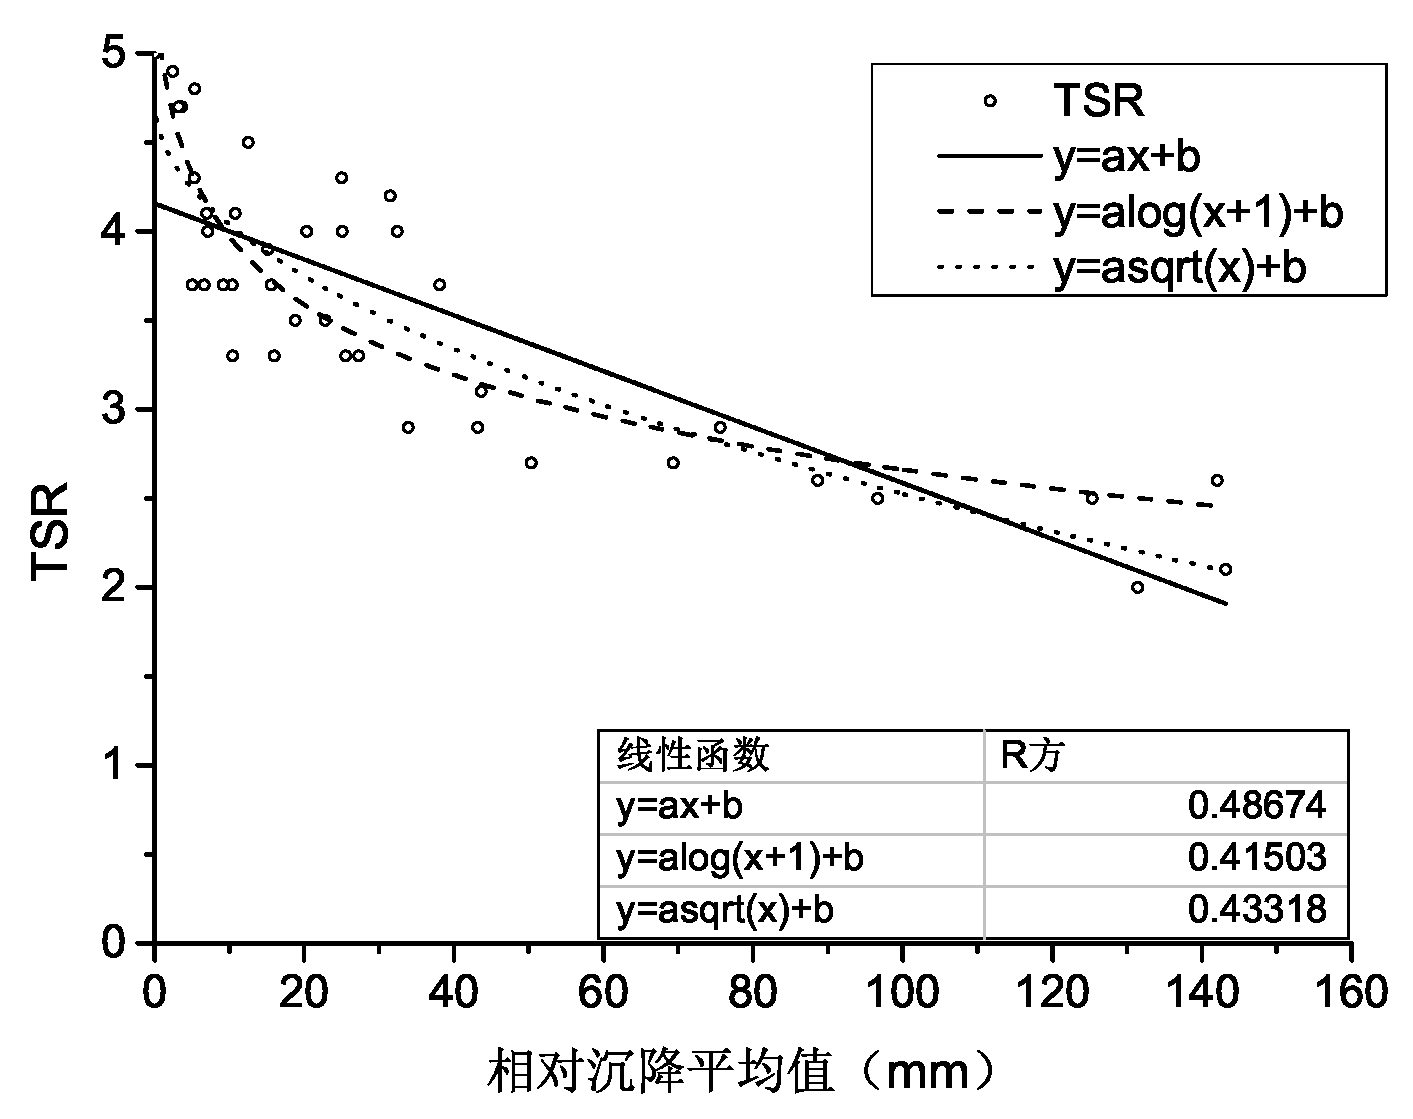
\includegraphics[width=0.48\textwidth]{chap2/tsr-setta.eps} & 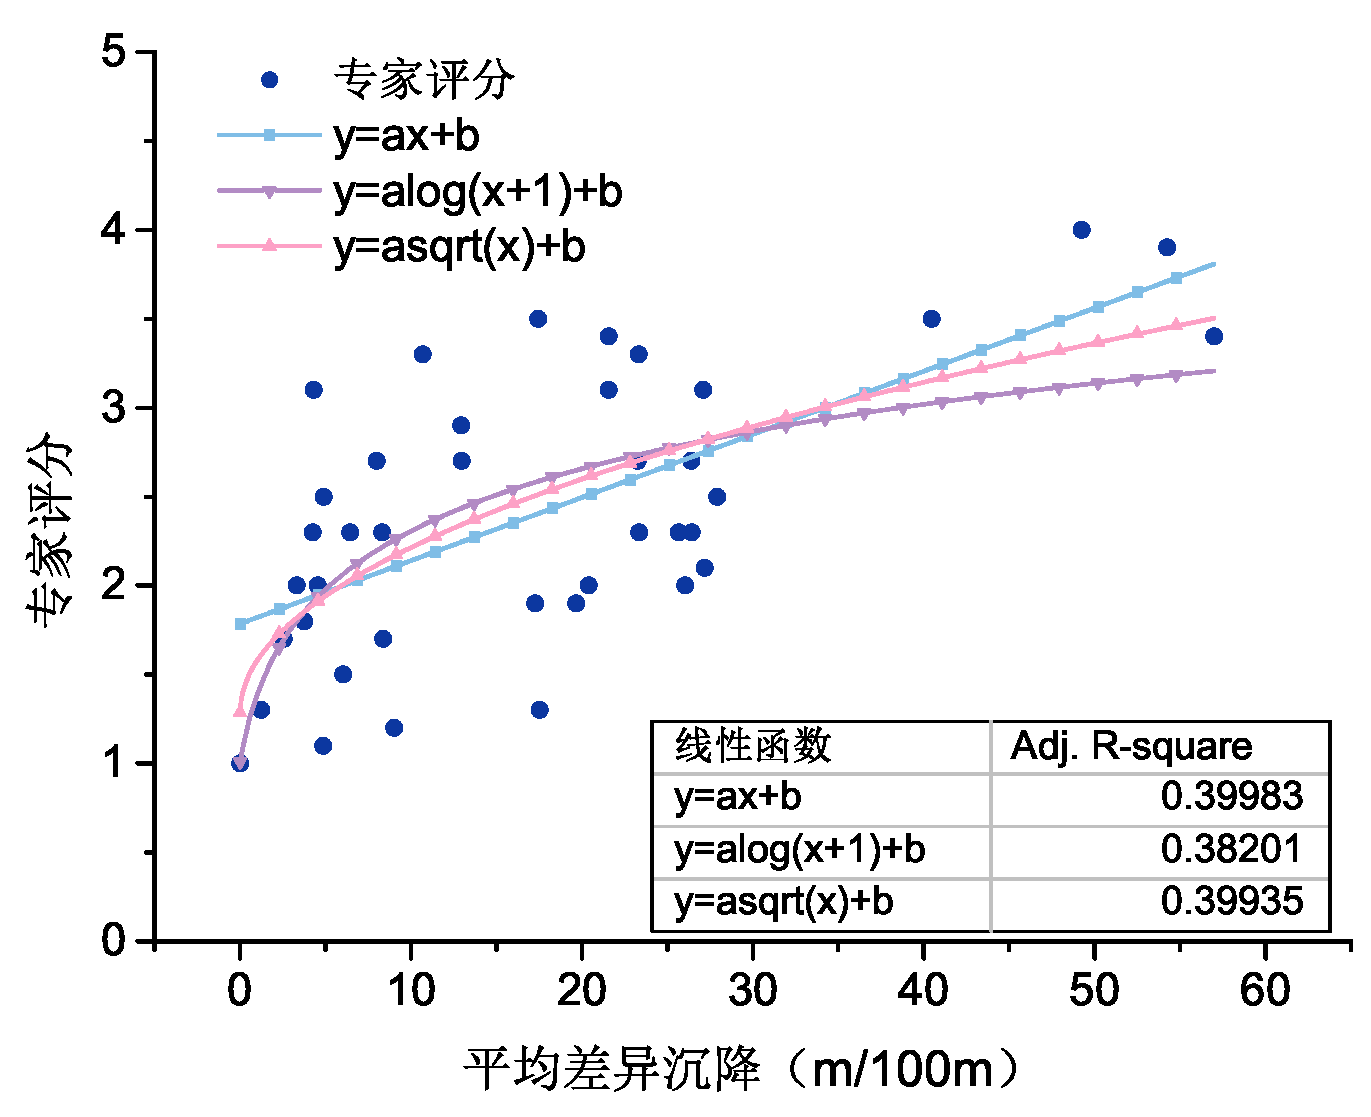
\includegraphics[width=0.48\textwidth]{chap2/tsr-settr.eps}\\ 
        (a)~TSR-${sett}_{a}$ & (b)~TSR-$set{{t}_{d\_a}}$\\
        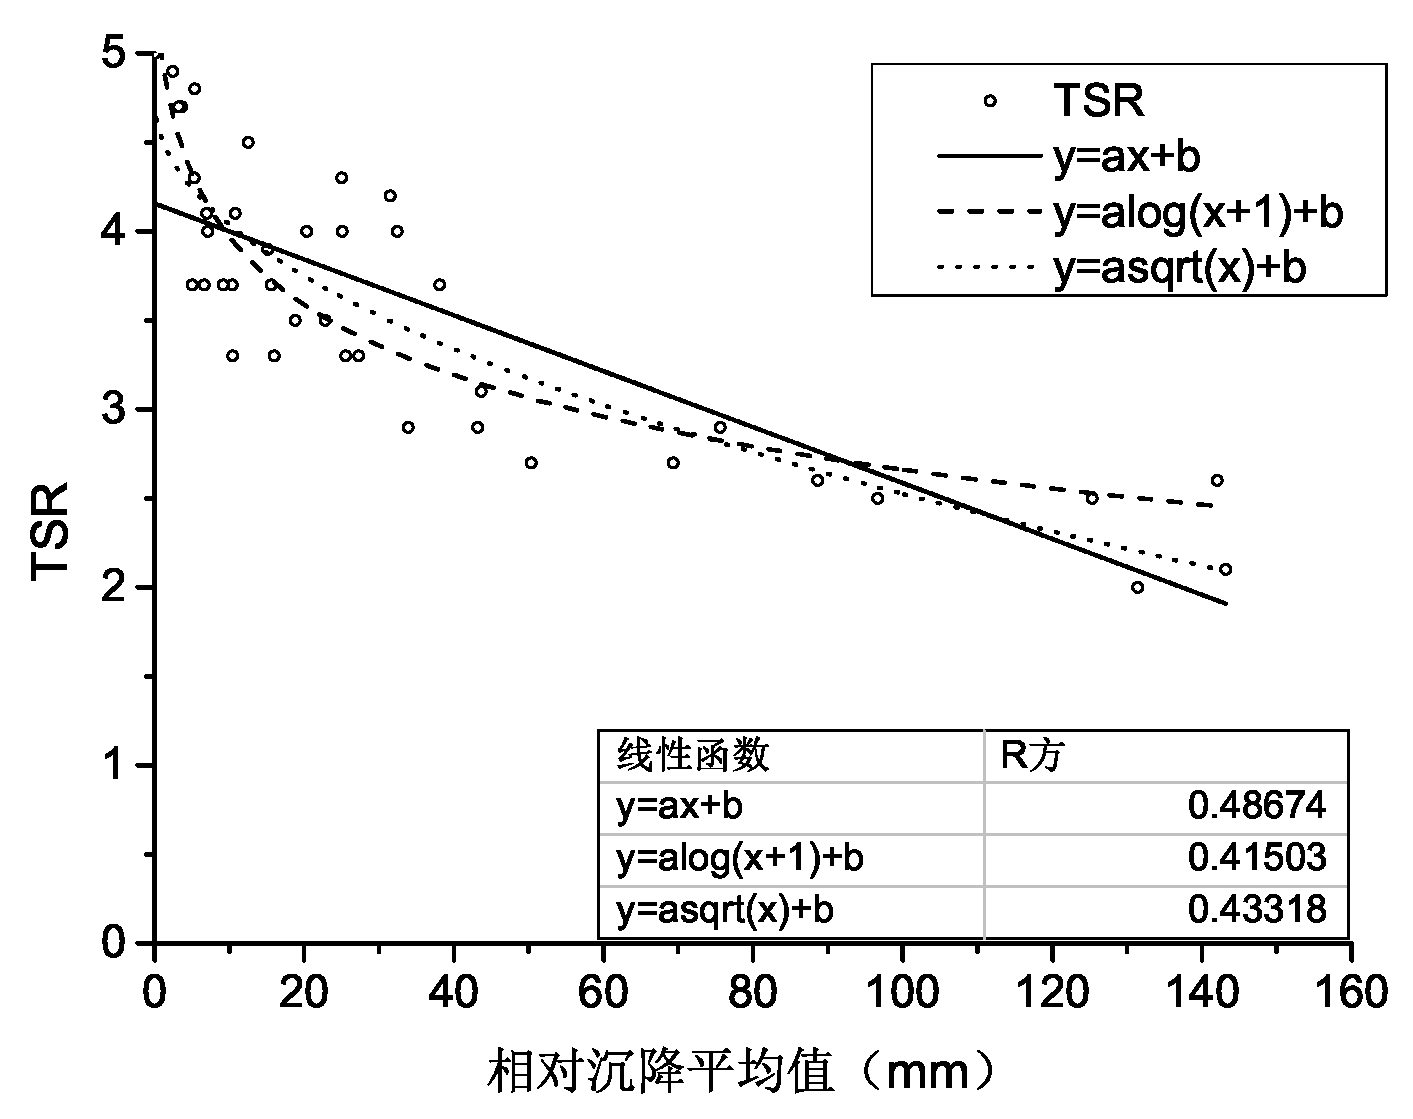
\includegraphics[width=0.48\textwidth]{chap2/tsr-setta.eps} & 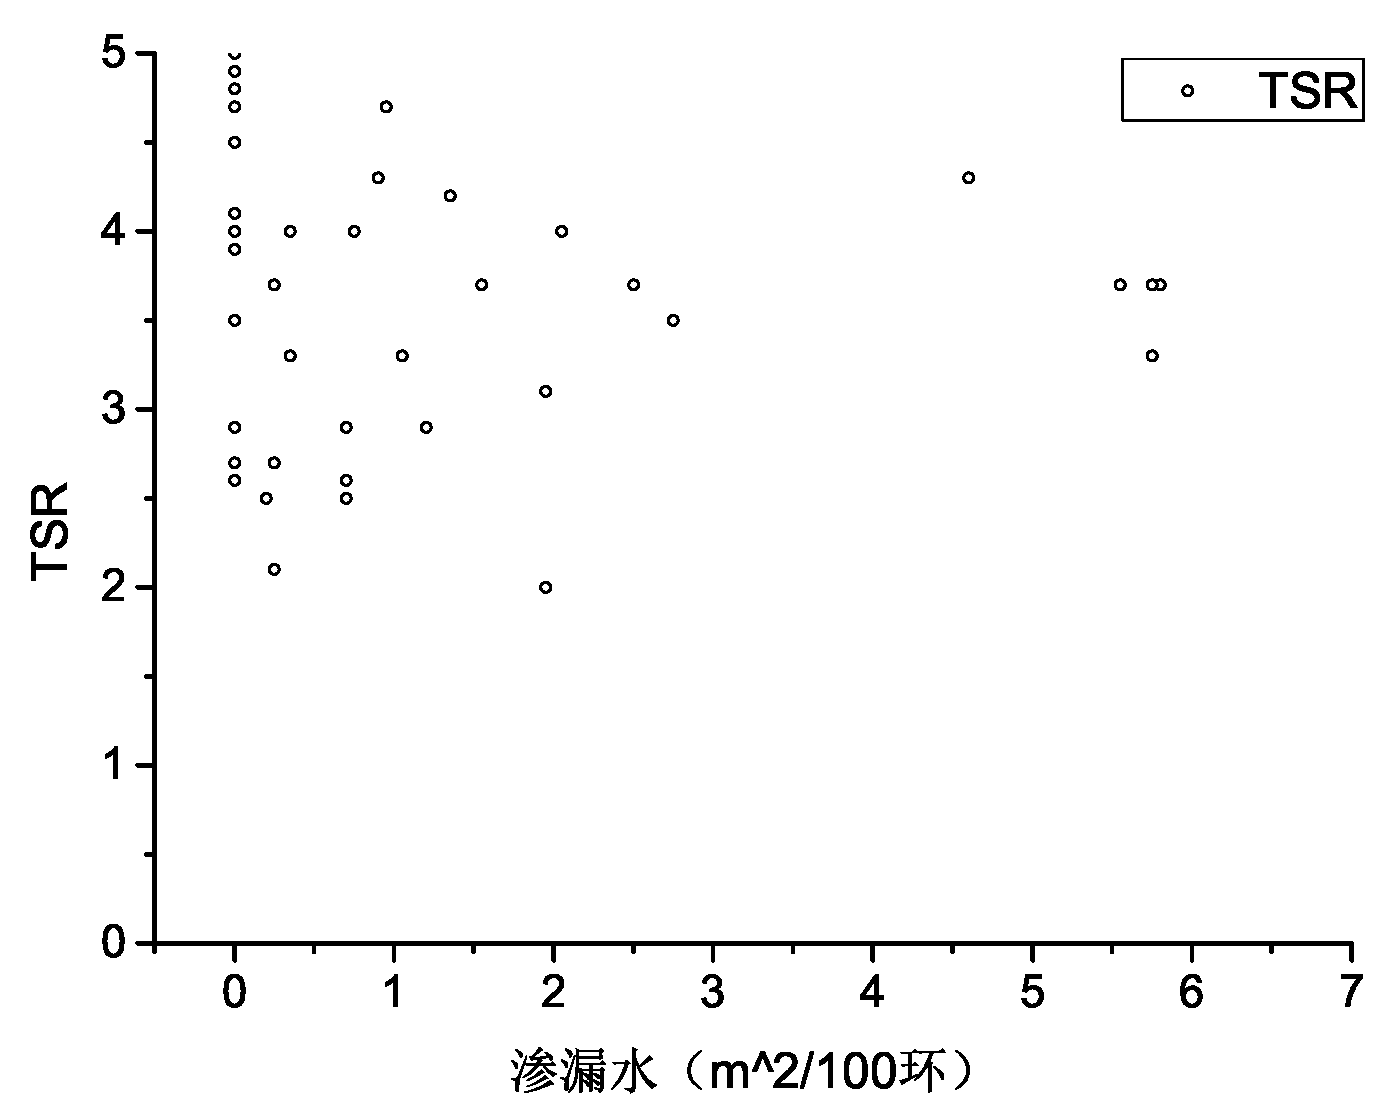
\includegraphics[width=0.48\textwidth]{chap2/tsr-leakge.eps}\\ 
        (c)~TSR-${cov}_{a}$ & (d)~TSR-${d}_{l}$\\
        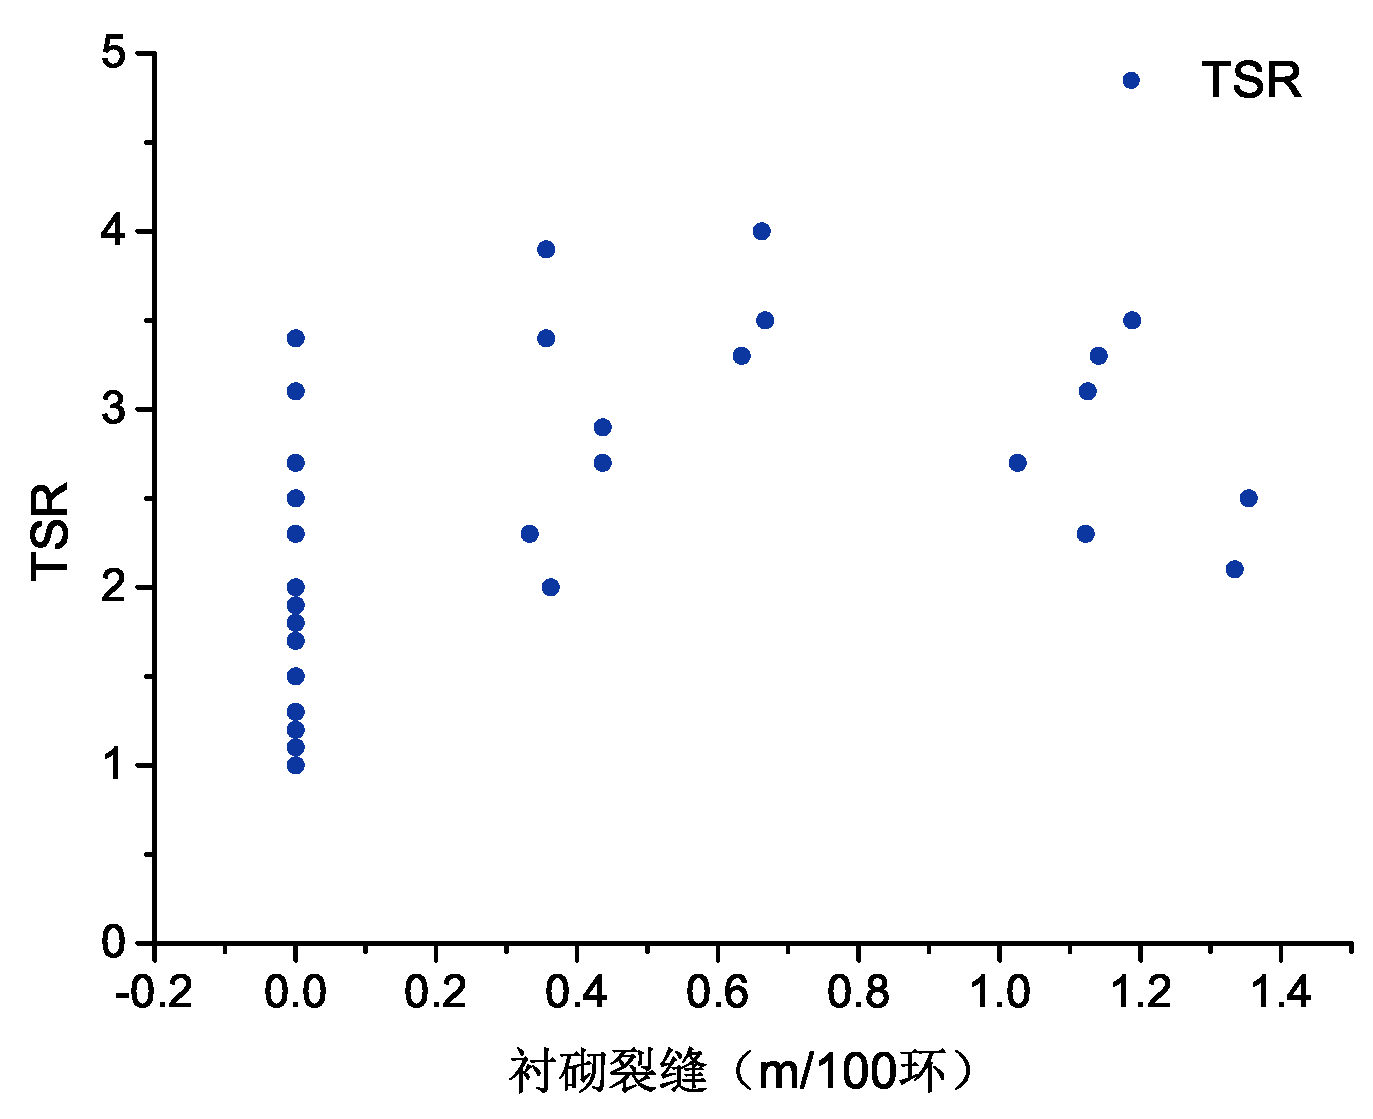
\includegraphics[width=0.48\textwidth]{chap2/tsr-spall.eps} & 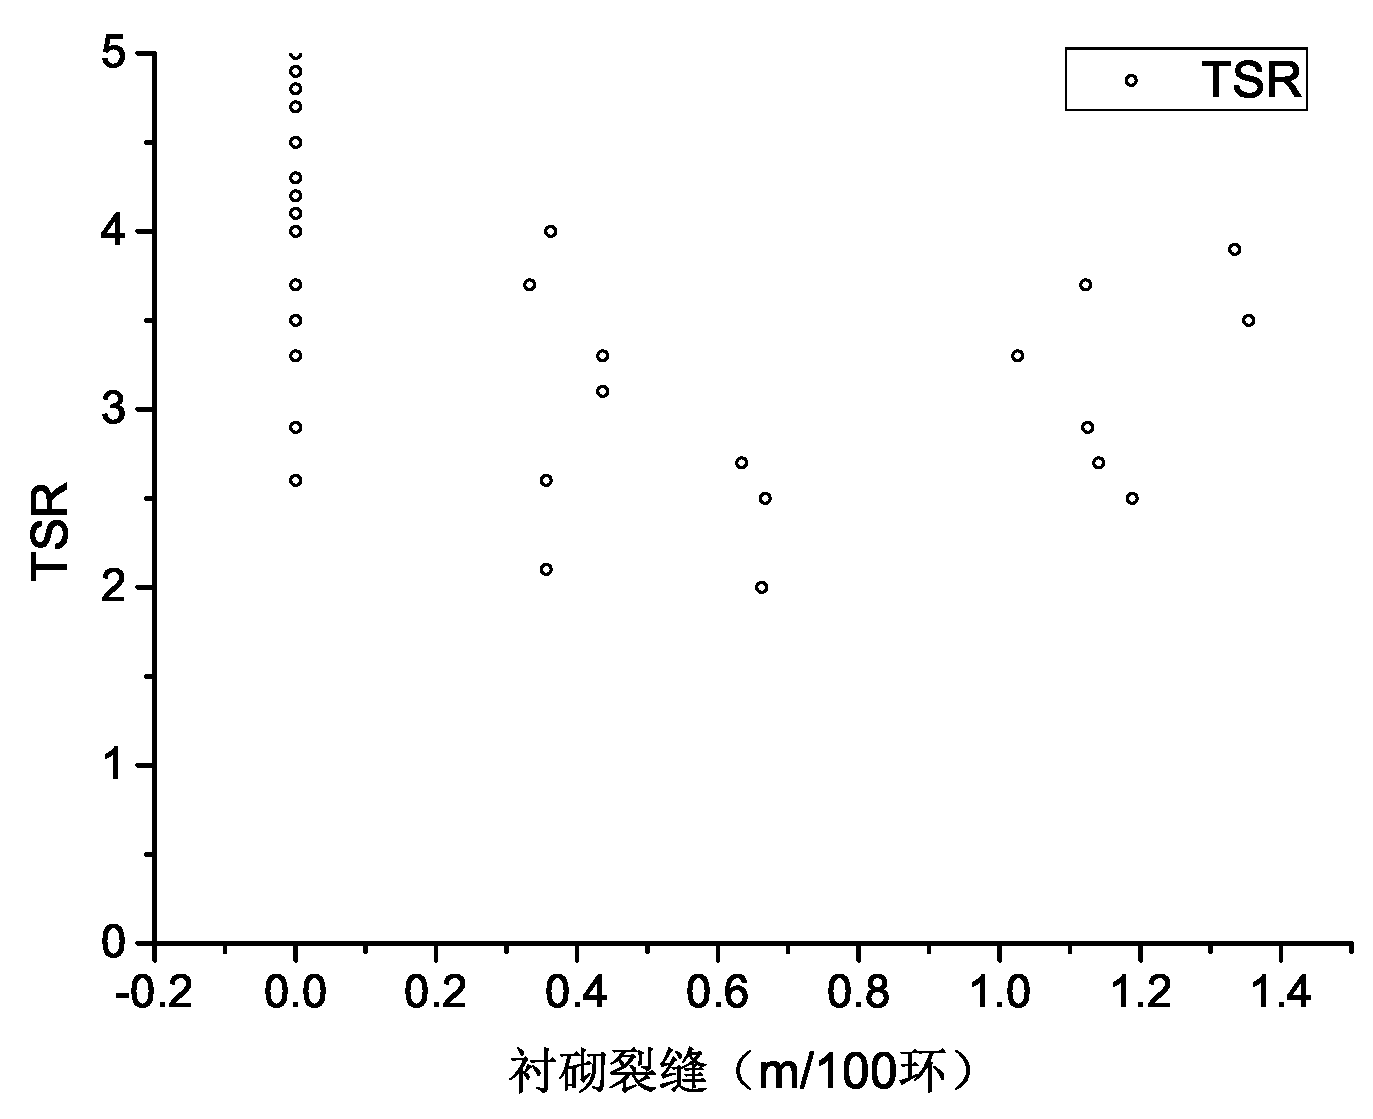
\includegraphics[width=0.48\textwidth]{chap2/tsr-crack.eps}\\ 
        (e)~TSR-$d_s$ & (f)~TSR-$d_c$\\
    \end{tabular}
    \caption{TSR与观测变量关系图} 
    \label{fig:TSR与观测变量关系图} 
\end{figure}

%+++++++++++++++++++++++++++++++++++++++++++++++++++++++++++++++++%
\subsection{偏最小二乘多元线性回归方法}

一般地,多元线性回归模型的自变量的基本要求是:在模型中应包含所有对因变量有重要解析意义的因素,并且自变量之间不存在线性相关的现象。若自变量之间存在严重的线性相关性,普通的最小二乘法拟合回归模型将不能保证回归结果的精确性和可靠性。而偏最小二乘回归能较好解决这一问题,其结合了主成分分析和典型相关性分析理论,能够在自变量存在相关性的条件下进行回归建模,同时更易识别系统信息与噪声。

偏最小二乘法的主要思想如下:设有$q$个因变量$\{{{y}_{1}},{{y}_{2}},\cdots ,{{y}_{q}}\}$和$p$个自变量$\{{{x}_{1}},{{x}_{2}},\cdots ,{{x}_{p}}\}$,为了研究因变量与自变量的统计关系,假设收集$n$个样本,则构成的自变量和因变量空间为$X={{[{{x}_{1}},\cdots ,{{x}_{p}}]}_{n\times p}}$和$Y={{[{{y}_{1}},\cdots ,{{y}_{q}}]}_{n\times q}}$。偏最小二乘是从$X$和$Y$中提取主成分$t_1$和$u_1$,即$t_1$是${{x}_{1}},\cdots ,{{x}_{p}}$的线性组合,$u_1$是${{y}_{1}},\cdots ,{{y}_{q}}$的线性组合,再进行线性回归时应满足下述两个要求:

(1)$t_1$和$u_1$应尽可能的携带$X$和$Y$中的变异信息;

(2)$t_1$和$u_1$之间的相关程度应尽可能大。

上述两个要求表明,$t_1$和$u_1$应尽可能好的代表数据$X$和$Y$,同时$t_1$对$u_1$又有较强的解释能力。在第一个成分被提取后,分别实施$X$对$t_1$和$Y$对$u_1$的回归。如果回归方程已经达到满意的精度,则得到结果;否则,利用$X$去除$t_1$的残余信息和$Y$去除$u_1$的残余信息循环进行成分提取,直到结果满意为止。下面简略说明偏最小二乘法的计算推导,更详细的推导内容可以参考相关书籍(Tobias,\citeyear{tobias1995introduction};王慧文,\citeyear{王惠文1999偏最小二乘回归方法及其应用})。

第一步:记${{E}_{0}}={{({{E}_{01}},\cdots ,{{E}_{0p}})}_{n\times p}}$为$X$经标准化处理后的矩阵,${{F}_{0}}={{({{F}_{01}},\cdots ,{{F}_{0q}})}_{n\times q}}$为$Y$经标准化处理后的矩阵;记$t_1$为${{E}_{0}}$第一主成分,$t_1={E_0}{w_1}$,$w_1$为$E_0$第一个轴,且$\left\| {{w}_{1}} \right\|=1$;记$u_1$为${{F}_{0}}$第一主成分,$u_1={F_0}{c_1}$,$c_1$为$F_0$第一个轴,且$\left\| {{c}_{1}} \right\|=1$。

如果要$t_1$、$u_1$能分别很好地代表$X$、$Y$中的数据变异信息,根据主成分分析原理(Wold,\citeyear{wold1987principal}),可得
\begin{align}
    \label{equ:variance1}
    Var({{t}_{1}})\to \max \\
    \label{equ:variance2}
    Var({{u}_{1}})\to \max
\end{align}
另一方面,要求$t_1$对$u_1$有最大的解释能力,根据典型相关分析理论(Thompson,\citeyear{thompson2005canonical}),$t_1$和$u_1$的相关度应达到最大,即
\begin{equation}
    \label{equ:relation}
    r({{t}_{1}},{{u}_{1}})\to \max 
\end{equation}
综上所示,即要求$t_1$对$u_1$的协方差最大,有
\begin{equation}
    \label{equ:relation}
    Cov({{t}_{1}},{{u}_{1}})=\sqrt{Var({{t}_{1}})Var({{u}_{1}})}r({{t}_{1}},{{u}_{1}})\to \max =\max \left\langle {{t}_{1}},{{u}_{1}} \right\rangle
\end{equation}

记${{\theta }_{1}}\text{=}\left\langle {{t}_{1}},{{u}_{1}} \right\rangle =\left\langle {{E}_{0}}{{w}_{1}},{{F}_{0}}{{c}_{1}} \right\rangle$,根据拉格朗日算法可推导出,$w_1$是矩阵${{{E}'}_{0}}{{F}_{0}}{{{F}'}_{0}}{{E}_{0}}$的特征向量,对应的特征值为$\theta _{1}^{2}$。根据式~\ref{equ:relation}~可知$\theta _{1}$要求取值最大,故$w_1$是对应矩阵${{{E}'}_{0}}{{F}_{0}}{{{F}'}_{0}}{{E}_{0}}$最大特征值的单位特征向量,同理$c_1$是对应矩阵${{{F}'}_{0}}{{E}_{0}}{{{E}'}_{0}}{{F}_{0}}$最大特征值的单项特征向量。

求得轴$w_1$和$c_1$后,即可得到成分
\begin{align}
    \label{equ:pc1}
    t_1={E_0}{w_1} \\
    \label{equ:pc2}
    u_1={F_0}{c_1}
\end{align}
然后可分别求$E_0$和$F_0$对$t_1$的回归方程
\begin{align}
    \label{equ:regress1}
    E_0={t_1}{p'_1}+E_1 \\
    \label{equ:regress2}
    F_0={t_1}{r'_1}+F_1
\end{align}
式中:$E_1$和$F_1$为残差矩阵;回归系数向量是
\begin{align}
    \label{equ:regress-index1}
    {{p}_{1}}=\frac{{{{{E}'}}_{0}}{{t}_{1}}}{{{\left\| {{t}_{1}} \right\|}^{2}}} \\
    \label{equ:regress-index2}
    {{r}_{1}}=\frac{{{{{F}'}}_{0}}{{t}_{1}}}{{{\left\| {{t}_{1}} \right\|}^{2}}}
\end{align}
    
第二步:用残差矩阵$E_1$和$F_1$取代$E_0$和$F_0$,求第二个轴$w_2$和$c_2$和第二个主成分$t_2$和$u_2$,同理第一步,可求出
\begin{align}
    \label{equ:regress3}
    E_1={t_2}{p'_2}+E_2 \\
    \label{equ:regress4}
    F_1={t_2}{r'_2}+F_2
\end{align}

如此计算下去,如果$X$的秩为$A$,最终可得
\begin{align}
    \label{equ:regress5}
    {{E}_{0}}={{t}_{1}}{{{p}'}_{1}}+\cdots +{{t}_{A}}{{{p}'}_{A}} \\
    \label{equ:regress6}
    {{F}_{0}}={{t}_{1}}{{{r}'}_{1}}+\cdots {{t}_{A}}{{{r}'}_{A}}+{{F}_{A}}
\end{align}

由于$t_1,\cdots ,t_A$均可以表示成${E}_{01},\cdots ,{E}_{0p}$的线性组合,因此式~\ref{equ:regress6}~可以写成$y_k=F_{0k}$关于$x_j=E_{0j}$的线性回归方程,即
\begin{equation}
    \label{equ:regress7}
    {{y}_{k}}={{a}_{k1}}{{x}_{1}}+\cdots +{{a}_{kp}}{{x}_{p}}+{{F}_{Ak}},k=1,2,\cdots ,q
\end{equation}
式中:$y_k$为矩阵$Y$的第$k$列;$a_{ki}$为$y_k$对应第$i$个自变量的系数;${F}_{Ak}$是残差矩阵$F_A$的第$k$列。

第三步:交叉有效性验证。首先将全部$n$个样本分成两个部分,第一部分是除去某个样本点$i$的其他样本点集合,用这部分样本点采用$h$个成分拟合回归方程;第二部分则把除去的一个样本点$i$带入拟合回归方程,得到$y_i$在样本$i$的拟合值${{\hat{y}}_{hj(-i)}}$。对于所有样本重复上述过程,可定义$y_i$的预测误差平方和为
\begin{equation}
    \label{equ:press}
    PRES{{S}_{hj}}=\sum\limits_{t=1}^{n}{\left( {{y}_{ij}}-{{{\hat{y}}}_{hj\text{-}i}} \right)}
\end{equation}
定义$Y$的预测误差平方和为
\begin{equation}
    {{PRESS}_{h}}=\sum\limits_{j=1}^{p}{{{PRESS}_{hj}}}
\end{equation}

另外,再采用所有样本点,拟合$h$个成分的回归方程。记第$i$个样本的预测值为${{\hat{y}}_{hji}}$,可以定义$y_j$的误差平方和为
\begin{equation}
    S{{S}_{hj}}=\sum\limits_{i=1}^{n}{{{\left( {{y}_{ij}}-\hat{y}_{hji} \right)}^{2}}}
\end{equation}
定义$Y$的误差平方和为
\begin{equation}
    S{{S}_{h}}=\sum\limits_{j=1}^{p}{S{{S}_{hj}}}
\end{equation}

对于全部因变量$Y$,成分$t_h$的交叉有效性定义为
\begin{equation}
    Q_{h}^{2}=1-\frac{\sum\limits_{k=1}^{q}{PRES{{S}_{hk}}}}{\sum\limits_{k=1}^{q}{S{{S}_{(h-1)k}}}}=1-\frac{PRES{{S}_{h}}}{S{{S}_{(h-1)}}}
\end{equation}
一般认为,当$Q_{h}^{2}\ge (1-{{0.95}^{2}})=0.0975$时,添加$t_h$对拟合效果的贡献是显著的。对于$k=1,2,\cdots ,q$,至少有一个$k$,使得
\begin{equation}
    Q_{hk}^{2}\ge 0.0975
\end{equation}
这时增加成分$t_h$,至少使得一个$y_k$的拟合模型得到显著的改善,因此可以考虑增加一个主成分$t_h$。

%+++++++++++++++++++++++++++++++++++++++++++++++++++++++++++++++++%
\subsection{TSI公式计算}

根据表~\ref{tab:隧道服役性能评分结果}~的评分结果和线性化处理结果,取$X=\left[ \sqrt{set{{t}_{a}}},set{{t}_{d\_a}},{{\operatorname{cov}}_{a}},{{d}_{l}},{{d}_{c}},{{d}_{s}} \right]$,$Y=\left[ TSR \right]$,偏最小二乘回归结果应为
\begin{gather}
    TSR={{A}_{1}}\sqrt{set{{t}_{a}}}+{{A}_{2}}set{{t}_{d\_a}}+{{B}_{1}}{{\operatorname{cov}}_{a}}+{{C}_{1}}{{d}_{l}}+{{C}_{2}}{{d}_{c}}+{{C}_{3}}{{d}_{s}}+C+{{F}_{k}} \\ 
    TSI={{A}_{1}}\sqrt{set{{t}_{a}}}+{{A}_{2}}set{{t}_{d\_a}}+{{B}_{1}}{{\operatorname{cov}}_{a}}+{{C}_{1}}{{d}_{l}}+{{C}_{2}}{{d}_{c}}+{{C}_{3}}{{d}_{s}}+C \\ 
    TSI=TSI+{{F}_{k}}
\end{gather}
式中:$A_1$,$A_2$,$B_1$,$C_1$,$C_2$,$C_3$和$C$均为待评估的系数;$F_k$为回归模型不能解释的残差。由于隧道变形和病害的增多,必然造成隧道服役性能的降低,故在物理意义上应为负数。

根据式~\ref{equ:regress1}-\ref{equ:regress-index2}~可计算得TSI的标准化公式
\begin{align}
  \label{tsi-std}
  & TS{I}'=-0.62\sqrt{set{{{{t}'}}_{a}}}-0.13set{{{{t}'}}_{d\_a}}-0.25\operatorname{co}{{{{v}'}}_{a}} \\ 
 & \quad \quad \quad -0.19{{{{d}'}}_{l}}-0.06{{d}_{c}}^{\prime }-0.03{{{{d}'}}_{s}} \nonumber
\end{align}
式中:${set{{{{t}'}}_{a}}}$,$set{{{t}'}_{d\_a}}$,${co}{{{v}'}_{a}}$,${{d}'_{c}}$,${{{d}'}_{s}}$分别为${set{{t}_{a}}}$,$set{{t}_{d\_a}}$,${{\operatorname{cov}}_{a}}$,${{d}_{l}}$,${{d}_{c}}$,${{d}_{s}}$的标准化公式。本文采取的标准公式如式~\ref{equ:标准化公式}~所示,其中$\mu$为样本的平均值,$\delta$为样本的标准差,根据表~\ref{tab:隧道服役性能评分结果}~可得公式~\ref{equ:tsi标准化}-\ref{equ:ds标准化}
\begin{gather}
 \label{equ:标准化公式} 
    {v}'=\frac{v-\mu }{\delta }\\
  \label{equ:tsi标准化}
    TS{I}'=\frac{TSI-{{\mu }_{TSI}}}{{{\delta }_{TSI}}}=\frac{TSI-3.6}{0.8} \\ 
  \label{equ:setta标准化}
    \sqrt{set{{{{t}'}}_{a}}}=\frac{\sqrt{set{{t}_{a}}}-{{\mu }_{setta}}}{{{\delta }_{setta}}}=\frac{\sqrt{set{{t}_{a}}}-5.2}{3.1} \\ 
 \label{equ:settda标准化}
    set{{{{t}'}}_{d\_a}}=\frac{set{{t}_{d\_a}}-{{\mu }_{settda}}}{{{\delta }_{settda}}}=\frac{set{{t}_{d\_a}}-17.2}{13.4} \\ 
 \label{equ:cova标准化}
    \operatorname{co}{{{{v}'}}_{a}}=\frac{{{\operatorname{cov}}_{a}}-{{\mu }_{\operatorname{cov}a}}}{{{\delta }_{\operatorname{cov}a}}}=\frac{{{\operatorname{cov}}_{a}}-6.1}{2.2} \\ 
 \label{equ:dl标准化}
    {{{{d}'}}_{l}}=\frac{{{d}_{l}}-{{\mu }_{dl}}}{{{\delta }_{dl}}}=\frac{{{d}_{l}}-1.3}{1.8} \\ 
 \label{equ:dc标准化}
    {{{{d}'}}_{c}}=\frac{{{d}_{c}}-{{\mu }_{dc}}}{{{\delta }_{dc}}}=\frac{{{d}_{c}}-0.5}{0.9} \\ 
 \label{equ:ds标准化}
    {{{{d}'}}_{s}}=\frac{{{d}_{s}}-{{\mu }_{ds}}}{{{\delta }_{ds}}}=\frac{{{d}_{s}}-0}{0.1}
\end{gather}


将原始数据带入式~\ref{tsi-std}~有
\begin{align}
  \label{tsi}
  & TSI=5.23-0.16\sqrt{set{{t}_{a}}}-0.01set{{t}_{d\_a}}-0.09{{\operatorname{cov}}_{a}} \\ 
 & \quad \quad \quad -0.08{{d}_{l}}-0.05{{d}_{c}}-0.50{{d}_{s}} \nonumber 
\end{align}

由标准化公式~\ref{tsi-std}~可知,累积沉降平均值指标所占比重对大,权重系数为0.62,即其在六个指标当中是最重要的,其次为平均收敛率、渗漏水、平均差异沉降。衬砌剥落和衬砌裂缝两个指标的权重较小,主要原因是专家认为目前上海地铁盾构隧道的大部分剥落和裂缝病害并不是运营期间产生的,而是由于施工期的不当操作造成,且在运营期这类病害并没有劣化的趋势。图~\ref{fig:TSI和TSR的比较与关系}~所示为评分样本的TSI和TSR关系与比较。图~\ref{fig:TSI和TSR的比较与关系}a~描述了公式~\ref{tsi}~的拟合度,$R^2$为$0.841$,即公式~\ref{tsi}~解释了84.1\%的评分样本数据。图~\ref{fig:TSI和TSR的比较与关系}b~所示为样本的TSI计算值与TSR值比较,图中可以看出,除了1号样本和15号样本,其余样本的TSI与TSR差值均在0.5以内。

\begin{figure}[htb!] 
    \centering 
    \begin{tabular}{c} 
        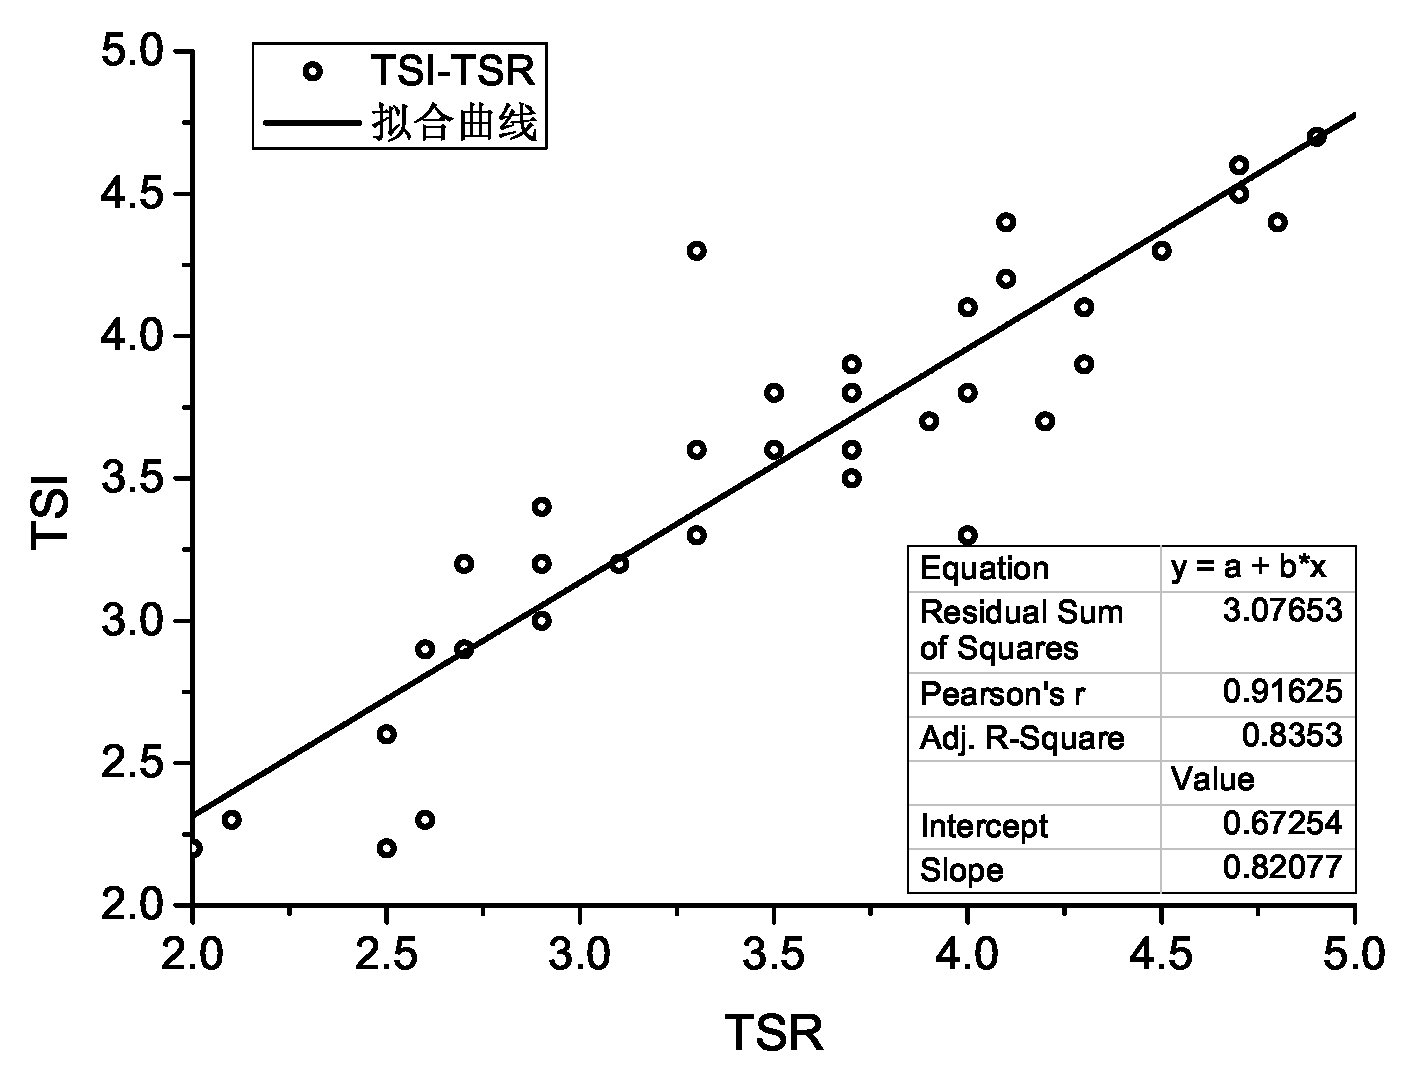
\includegraphics[width=0.7\textwidth]{chap2/tsi-tsr.eps} \\ 
        (a)~TSI和TSR关系图 \\
        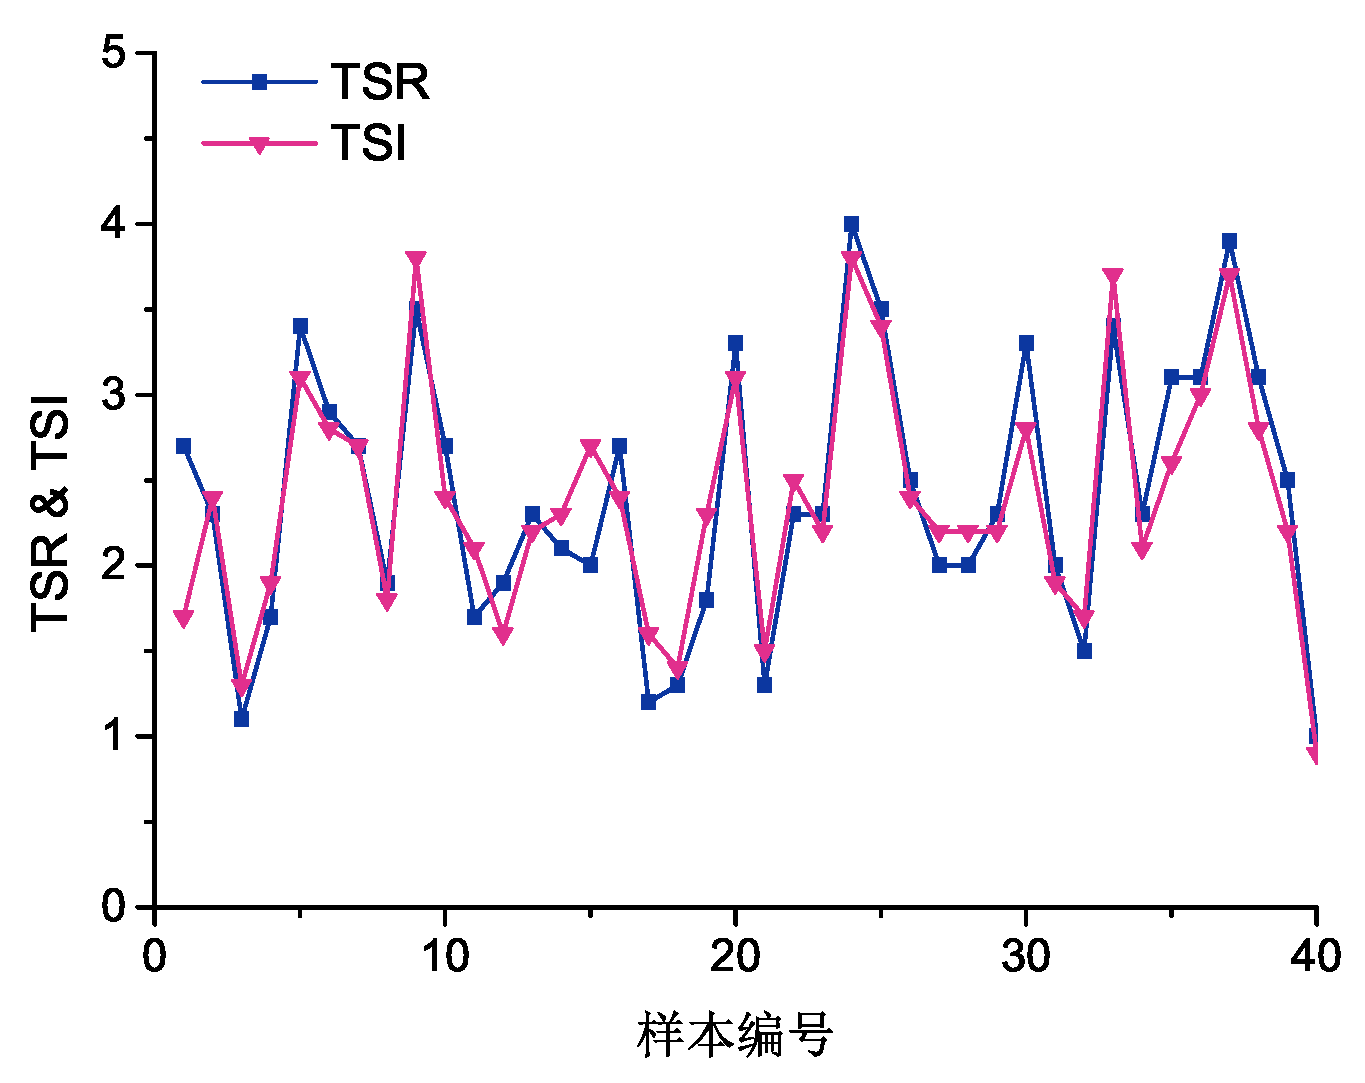
\includegraphics[width=0.65\textwidth]{chap2/tsitsr-no.eps} \\ 
        (b)~评分样本的TSI和TSR比较 \\
    \end{tabular}
    \caption{评分样本TSI和TSR的比较与关系} 
    \label{fig:TSI和TSR的比较与关系} 
\end{figure}

%%%%%%%%%%%%%%%%%%%%%%%%%%%%%%%%%%%%%%%%%%%%%%%%%%%%%%%%%%%%%%%%%%%
\section{盾构隧道服役性变权修正}

公式~\ref{tsi}~给出了TSI与评估指标之间的线性关系,每个指标的权重系数均为固定常数。对于实际盾构隧道,若有一指标值较大,则该指标的进一步劣化对服役性能的影响变得十分重要,具有明显的“木桶效应”。常数权重则不能反映这一现象,对指标灵敏性、动态环境的适应性低。

动态变权首先需要考虑指标的劣化程度。以盾构隧道的累积沉降为例,在相同时间内新增相同的沉降,对累积沉降已经较大的隧道的影响要比累积沉降相对较小的隧道,数学上称这种特性为悲观性(李蓉,\citeyear{李蓉2007基于层次分析法的桥梁健康状态模糊综合评估方法的研究及其应用}),其数学公式为
\begin{equation}
    g=G(v)=\left\{ \begin{matrix}
   1-\left( \frac{v-{{v}_{\min }}}{{{v}_{\max }}-{{v}_{\min }}} \right){{e}^{\frac{v-{{v}_{\min }}}{{{v}_{\max }}-{{v}_{\min }}}-1}}\quad {{v}_{\max }}\ge v\ge {{v}_{\min }}  \\
   0\quad \quad \quad \quad \quad \quad \quad v>{{v}_{\max }}  \\
\end{matrix} \right.
\end{equation}
式中:$g$为指标健康度,$g$越小代表指标越严重;$v$为指标的值;$v_min$为指标的下限值;$v_max$为指标的上限值。曲线如图~\ref{fig:悲观型曲线图}~所示。

\begin{figure}[htb!]
    \centering
    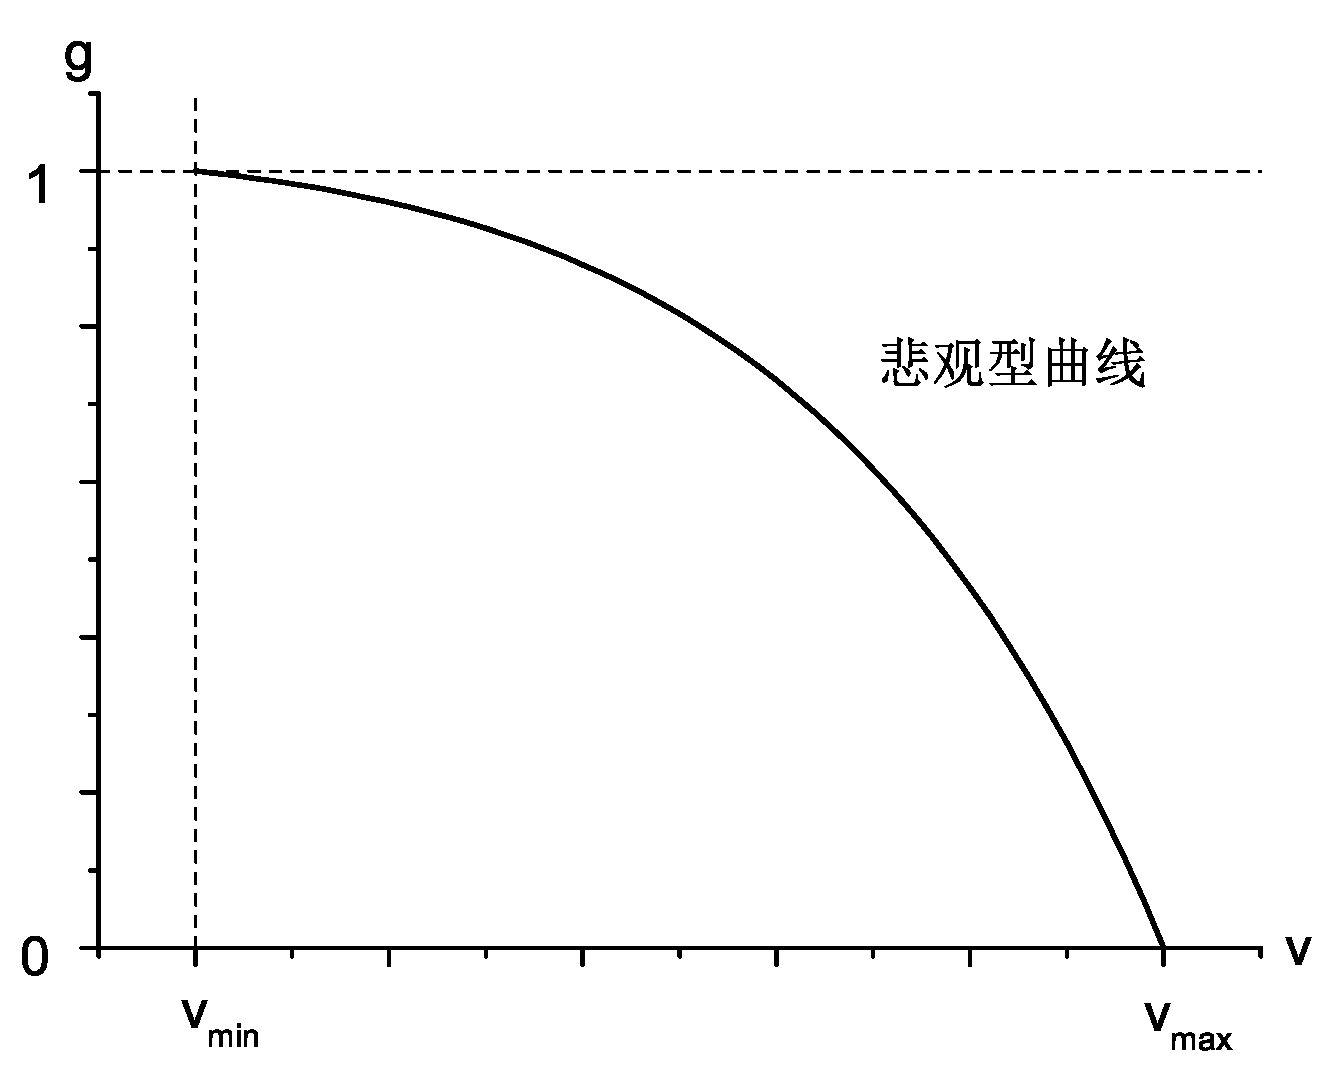
\includegraphics[width=0.7\textwidth]{chap2/stdline.eps}
    \caption{悲观型曲线图}
    \label{fig:悲观型曲线图}
\end{figure}

Cheng等(\citeyear{cheng1999evaluating})引入变权函数,采用变权权重替换常权权重,反映指标不同劣化程度在TSI计算时的重要程度不同。对于变权和状态函数的公理化定义如下:

定义一:一组变权$\mathbf{{w}'}(\mathbf{g})=\left( {{{{w}'}}_{1}}(\mathbf{g}),{{{{w}'}}_{2}}(\mathbf{g}),\cdots ,{{{{w}'}}_{n}}(\mathbf{g}) \right)$,指的是对应$n$个指标的映射${{{w}'}_{i}}(i=1,2,\cdots ,n)$,${{{w}'}_{i}}:({{g}_{1}},{{g}_{2}},\cdots ,{{g}_{n}})\mapsto {{{w}'}_{i}}({{g}_{1}},{{g}_{2}},\cdots ,{{g}_{n}})$,应满足:

(1)归一性:$\sum\limits_{i=1}^{n}{{{{{w}'}}_{i}}({{g}_{1}},\cdots ,{{g}_{n}})=1}$;

(2)连续性:${{{w}'}_{i}}({{g}_{1}},\cdots ,{{g}_{n}})(i=1,\cdots ,n)$对所有变元$g_i$是连续的;

(3)惩罚性:${{{w}'}_{i}}({{g}_{1}},\cdots ,{{g}_{n}})(i=1,\cdots ,n)$对所有变元$g_i$是单调下降的;

(3')激励性:${{{w}'}_{i}}({{g}_{1}},\cdots ,{{g}_{n}})(i=1,\cdots ,n)$对所有变元$g_i$是单调上升的;

(3'')混合性:${{{w}'}_{i}}({{g}_{1}},\cdots ,{{g}_{n}})(i=1,\cdots ,n)$对部分变元单调下降,对部分变元单调上升。

定义二:映射$\mathbf{g}\mapsto \mathbf{d}(\mathbf{g})=({{d}_{1}}(\mathbf{g}),\cdots ,{{d}_{n}}(\mathbf{g}))$,称$\mathbf{d}(\mathbf{g})$为一个$n$维变权向量,${d}(\mathbf{g})$为状态变权函数,其满足

(1)惩罚型:${{g}_{i}}\ge {{g}_{j}}\Rightarrow {{d}_{i}}(\mathbf{g})\le {{d}_{j}}(\mathbf{g})$;

(1')激励型:${{g}_{i}}\ge {{g}_{j}}\Rightarrow {{d}_{i}}(\mathbf{g})\ge {{d}_{j}}(\mathbf{g})$;

(2)${{d}_{i}}(\mathbf{g})(i=1,\cdots .n)$对所有变元$g_i$连续;

(3)对常权向量$\mathbf{w}=({{w}_{1}},\cdots ,{{w}_{n}})$,可构造变权公式
\begin{equation}
    \label{equ:状态变权函数}
    \mathbf{{w}'}(\mathbf{g})=\frac{({{w}_{1}}{{d}_{1}}(\mathbf{g}),\cdots ,{{w}_{n}}{{d}_{n}}(\mathbf{g})}{\sum\limits_{i=1}^{n}{({{w}_{i}}{{d}_{i}}(\mathbf{g}))}}=\frac{\mathbf{w}\cdot \mathbf{d}(\mathbf{g})}{\sum\limits_{i=1}^{n}{({{w}_{i}}{{d}_{i}}(\mathbf{g}))}}
\end{equation}

公式~\ref{equ:状态变权函数}~最重要的是选择合适的状态变权函数,在数学上,常用的函数为幂函数形式(孙九春,\citeyear{孙九春2002大型桥梁综合评估系统研究}),如式~\ref{equ:幂函数变权函数}
\begin{equation}
    \label{equ:幂函数变权函数}
    {{d}_{i}}(\mathbf{g})={{(\frac{{{g}_{i}}}{100})}^{\varepsilon -1}}\quad 0<\varepsilon <1
\end{equation}

采用幂函数作为状态变权函数时,只有当指标接近指标上限时,权重变化才明显,变权灵敏度在指标发展前期仍然较低。而且式~\ref{equ:幂函数变权函数}~在$g=0$时奇异,也给计算带来不便。对于盾构隧道的实际情况,陈楠(\citeyear{陈楠2017考虑发展趋势与指标关联的隧道结构健康评估方法研究})提出采用分段状态变权函数替代幂函数
\begin{equation}
    \label{equ:分段状态变权函数}
    {{d}_{i}}(\mathbf{g})=\left\{ \begin{array}{*{35}{l}}
   {{m}^{4-5g}},0\le g\le 0.8  \\
   1,0.8\le g  \\
\end{array} \right.
\end{equation}
式中:$m$为形状参数,一般可取$m=2.5$。

图~\ref{fig:分段变权函数与幂函数变权函数比较}~描述了分段状态变权函数与幂函数状态变权函数的形状,由图可知,当某一指标的健康度$g$降低至0.8时,该指标所占权重将略微有所增加,当$g$继续降低至0.6-0.4时,所占权重将会有明显的增加,当$g$降低至0.2时,也就是一般单项指标预警值临界值时,指标权重将迅速增加,使该指标起决定作用。分段状态变权与幂函数变权公式相比,在指标发展早期有较好的预警效果。

\begin{figure}[htbp]
    \centering
    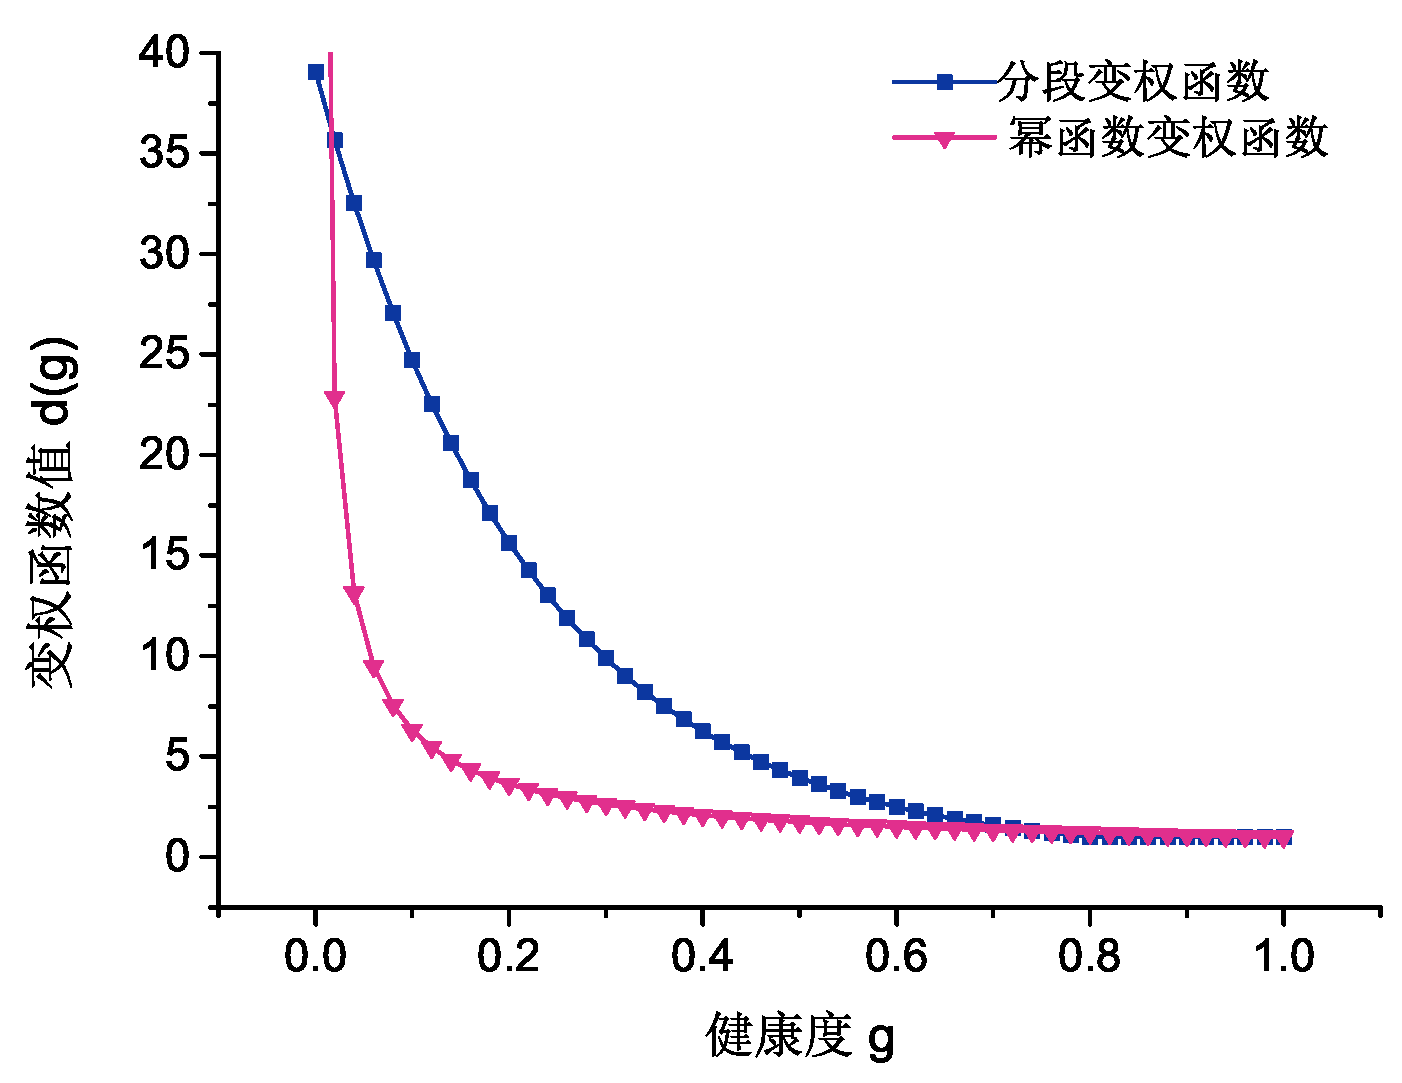
\includegraphics[width=0.7\textwidth]{chap2/dynamic-weight.eps}
    \caption{分段变权函数与幂函数变权函数比较}
    \label{fig:分段变权函数与幂函数变权函数比较}
\end{figure}

下面以具体数据为例,说明变权TSI计算过程。首先应确定各指标的允许最大值,采用朱宝林(\citeyear{朱宝林2014运营地铁盾构隧道状态评估及预测方法研究})对隧道病害分级的建议值,本文对六个评估指标的极限值取值如表~\ref{tab:评估指标允许最小和最大值}~所示。假设对于某段地铁区间的指标数值如表~\ref{tab:TSI变权函数计算过程}~第2列所示,根据公式~\ref{tsi-std}~可知TSI标准化公式的指标系数如第3列所示,根据系数计算各指标的权重,结果为第4列数据,根据指标数值计算指标的健康度,如第5列,根据公式~\ref{equ:分段状态变权函数}~得到变权函数值,如第6列,最后重新计算各指标的权重和标准化系数,分别如第7、8列所示。

\begin{table}[htbp]
  \centering
  \caption{评估指标允许最小和最大值}
    \begin{tabular}{?m{7em}<{\centering}"m{7em}<{\centering}"m{7em}<{\centering}?}
    \thickhline
    $v$     & \multicolumn{1}{c"}{$v_{min}$} & \multicolumn{1}{m{7em}<{\centering}?}{$v_{max}$} \bigstrut\\
    \thinhline
    $\sqrt{{sett}_{a}}$ & 0     & \multicolumn{1}{c?}{$\sqrt{60}$~$mm$} \bigstrut\\
    \thinhline
    ${sett}_{d\_a}$ & 0     & \multicolumn{1}{c?}{30~$mm/100m$} \bigstrut\\
    \thinhline
    ${cov}_{a}$   & 0     & \multicolumn{1}{c?}{12~$‰D$} \bigstrut\\
    \thinhline
    $d_l$    & 0     & \multicolumn{1}{c?}{1~$m^2$} \bigstrut\\
    \thinhline
    $d_c$    & 0     & \multicolumn{1}{c?}{0.5~$m$} \bigstrut\\
    \thinhline
    $d_s$    & 0     & \multicolumn{1}{c?}{0.5~$m^2$} \bigstrut\\
    \thickhline
    \end{tabular}%
  \label{tab:评估指标允许最小和最大值}%
\end{table}%

\begin{table}[htbp]
  \centering
  \caption{TSI变权函数计算过程}
    \begin{tabular}{?c"c"m{4em}<{\centering}"c"c"c"c"c?}
    \thickhline
    指标    & 数值  & 标准化方程系数 & 初始权重  & 健康度   & 变权函数 & 变权权重  & 变权系数 \bigstrut\\
    \thinhline
    $\sqrt{{sett}_{a}}$ & 3.7   & -0.62 & 0.48  & 0.98  & 1.00  & 0.47  & -0.60  \bigstrut\\
    \thinhline
    ${sett}_{d\_a}$ & 13.5  & -0.13 & 0.10  & 0.74  & 1.31  & 0.13  & -0.17  \bigstrut\\
    \thinhline
    ${cov}_{a}$   & 3.9   & -0.25 & 0.20  & 0.83  & 1.00  & 0.19  & -0.24  \bigstrut\\
    \thinhline
    $d_l$    & 0.35  & -0.19 & 0.15  & 0.82  & 1.00  & 0.14  & -0.18  \bigstrut\\
    \thinhline
    $d_c$    & 0     & -0.06 & 0.05  & 1.00  & 1.00  & 0.05  & -0.06  \bigstrut\\
    \thinhline
    $d_s$    & 0     & -0.03 & 0.02  & 1.00  & 1.00  & 0.02  & -0.03  \bigstrut\\
    \thickhline
    \end{tabular}%
  \label{tab:TSI变权函数计算过程}%
\end{table}%

根据公式~\ref{equ:setta标准化}-\ref{equ:ds标准化}~可计算得到各指标的标准化值分别为:-0.48、-0.28、-1.0、-0.04、0和0,根据更新后的指标系数,可计算标准化后的TSI
\begin{align}
  & TS{I}'=-0.60\sqrt{set{{{{t}'}}_{a}}}-0.17set{{{{t}'}}_{d\_a}}-0.24\operatorname{co}{{{{v}'}}_{a}} \nonumber \\ 
 & \quad \quad \quad -0.18{{{{d}'}}_{l}}-0.06{{d}_{c}}^{\prime }-0.03{{{{d}'}}_{s}} \nonumber \\ 
 & \quad \quad \; \text{=}-\text{0}\text{.60}\times (-0.48)-0.17\times (-0.28)-0.24\times (-1.0) \nonumber \\ 
 & \quad \quad \quad -0.18\times (-0.04)-0.06\times 0.0-0.03\times 0.0 \nonumber \\ 
 & \quad \quad =0.5828 \nonumber
\end{align}
再根据公式~\ref{equ:tsi标准化}~可计算得变权后的TSI值
\begin{equation}
    TSI=TS{I}'\times 0.8+3.6=4.1 \nonumber
\end{equation}

为了比较变权修正的TSI和常权TSI,在上述评估指标大小数值保持不变的情况下,增加平均收敛变形率,比较两种计算方法在某一指标不断劣化下的服役性能计算值。结果如图~\ref{fig:常权TSI与变权TSI曲线比较}~所示。对于常权TSI,不管指标劣化程度,单个指标的增加对TSI的影响都是一致的,对于变权TSI,随着指标的增加,在指标数值越大,其对TSI的影响越大,更符合实际情况。

\begin{figure}[htb!]
    \centering
    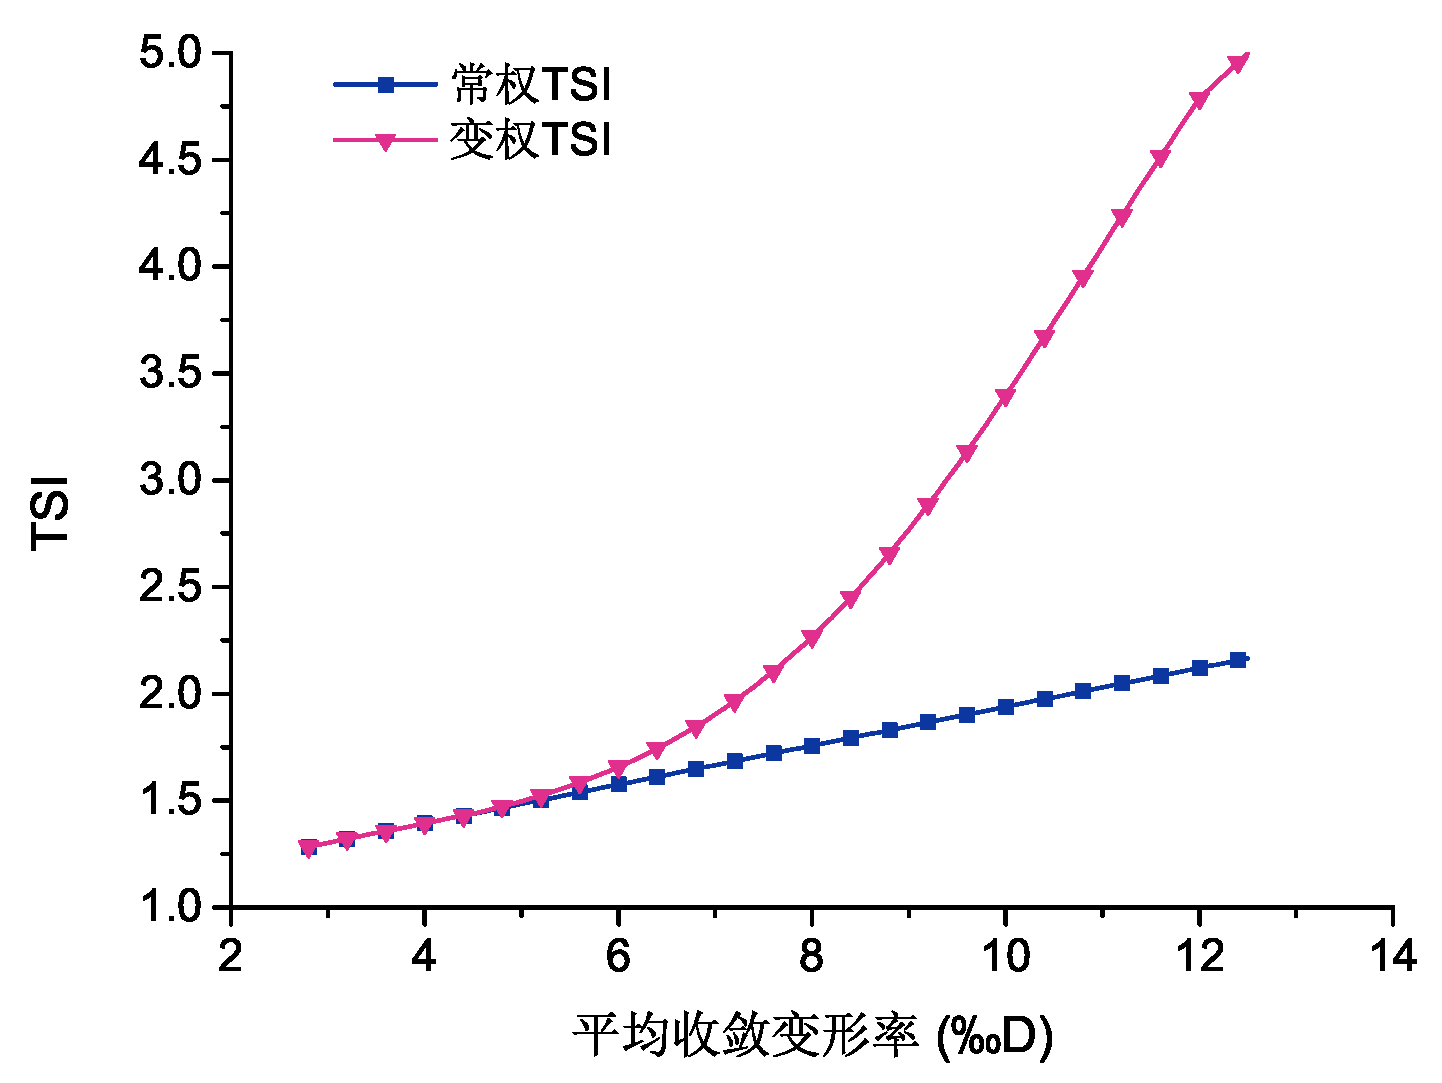
\includegraphics[width=0.7\textwidth]{chap2/const-change.eps}
    \caption{常权TSI与变权TSI曲线比较}
    \label{fig:常权TSI与变权TSI曲线比较}
\end{figure}

%%%%%%%%%%%%%%%%%%%%%%%%%%%%%%%%%%%%%%%%%%%%%%%%%%%%%%%%%%%%%%%%%%%
\section{本章小结}

本章提出了考虑评估指标相关性和指标劣化程度的变权服役性能评估方法,该评估方法具备物理意义明确、简单高效的特点,具体内容包括:

(1)给出了盾构隧道服役性能相关的基本概念定义,和本章评估方法的基本假设;

(2)根据现有监测和病害数据,结合数据之间的相关性,选取六个评估指标,分别为相对沉降平均值${sett}_{a}$、平均差异沉降$set{{t}_{d\_a}}$、平均收敛变形率${cov}_{a}$、百环渗漏水面积${d}_{l}$、百环衬砌剥落面积${d}_{s}$、百环裂缝长度${d}_{c}$。

(3)基于专家打分法和偏最小二乘法,回归拟合得出TSI计算公式如下,并给出根据指标劣化程度的TSI变权修正方法。
\begin{align}
  & TSI=5.23-0.16\sqrt{set{{t}_{a}}}-0.01set{{t}_{d\_a}}-0.09{{\operatorname{cov}}_{a}} \nonumber \\ 
 & \quad \quad \quad -0.08{{d}_{l}}-0.05{{d}_{c}}-0.50{{d}_{s}} \nonumber 
\end{align}

TSI计算方法已被国家行业标准《城市轨道交通隧道结构养护技术规范》所采纳。

